\documentclass[a4paper]{report}
\usepackage[group-separator={,},group-minimum-digits={3}]{siunitx}
\usepackage[utf8]{inputenc}
\usepackage[dvipsnames]{xcolor}
\usepackage{tcolorbox}
\usepackage{multicol}
\usepackage{lipsum}
\usepackage[margin=0.2in]{geometry}
\usepackage{xstring}
\usepackage{xifthen}
\usepackage[dvipsnames]{xcolor}
\usepackage{setspace}
\usepackage{amsmath}
\usepackage{enumitem}
\pagenumbering{gobble}
\setlength{\columnsep}{1.5cm}
\setlength{\columnseprule}{0.2pt}
\usepackage{hyperref}
\usepackage[none]{hyphenat}
\usepackage{graphicx}
\usepackage{etoolbox}
\usepackage{titlepic}
\usepackage[super]{nth}
\usepackage{setspace}
\usepackage{CJKutf8}
\usepackage[document]{ragged2e}

\hypersetup{
    colorlinks,
    citecolor=black,
    filecolor=black,
    linkcolor=black,
    urlcolor=black
}

\usepackage[default]{sourcesanspro}
\usepackage[T1]{fontenc}

\makeatletter
\def\@makechapterhead#1{%
  %\vspace*{5\p@}%
  {\parindent \z@ \raggedleft \normalfont
    \ifnum \c@secnumdepth >\m@ne
        \large\bfseries #1
        \par\nobreak
%        \vskip 10\p@
        \rule{\columnwidth}{.1pt}%
%        \vskip 10\p@
    \fi
    \interlinepenalty\@M
%    \large \bfseries \MakeUppercase{#1}\par\nobreak
%    \vskip 5\p@
  }}
\makeatother


\newcommand{\blitzloss}{\textbf{\textcolor{Magenta}{Blitz Loss}}}
\newcommand{\lostblitz}{\textbf{\textcolor{Magenta}{lost Blitz}}}

\newcommand{\blitzwin}{\textbf{\textcolor{OliveGreen}{Blitz Win}}}
\newcommand{\wonblitz}{\textbf{\textcolor{OliveGreen}{won Blitz}}}

\usepackage{enumitem}
\setitemize{noitemsep,topsep=0pt,parsep=0pt,partopsep=0pt}
\usepackage{graphicx}
\ifthenelse{%
		\equal{\blitzresult}{win}
	}{%
		\title{FFX Any\% - \blitzwin}
	}{%
		\ifthenelse{%
			\equal{\blitzresult}{loss}
		}{%
			\title{FFX Any\% - \blitzloss}
		}{%
			\ifthenelse
			}{}
		}
	}
\author{Mr.Tyton}
\titlepic{
\includegraphics[width=\textwidth]{final_fantasy_x_logo_by_eldi13_d4204zv}}
\begin{document}
\singlespacing
\maketitle
\tableofcontents

\makeatletter
\patchcmd{\chapter}{\if@openright\cleardoublepage\else\clearpage\fi}{}{}{}
\makeatother

\newenvironment{battle}[2][]{\begin{tcolorbox}[title=\begin{center}\MakeUppercase{#2} \ifthenelse{\isempty{#1}}{}{- \num{#1} HP}\end{center},colbacktitle=red!50!white,colframe=red!55,coltitle=black]}{\end{tcolorbox}}

\newenvironment{shop}[1]{\begin{tcolorbox}[title=\begin{center}SHOP\, #1 GIL\end{center},colbacktitle=blue!50!white,coltitle=black,colframe=blue!50!white]}{\end{tcolorbox}}

\newenvironment{spheregrid}{\begin{tcolorbox}[title=\begin{center}SPHERE GRID\end{center},colbacktitle=purple!50!white,colframe=purple!55,coltitle=black]}{\end{tcolorbox}}

\newenvironment{encounters}{\begin{tcolorbox}[title=\begin{center}ENCOUNTERS\end{center},colbacktitle=VioletRed!50!white,colframe=VioletRed!55,coltitle=black]}{\end{tcolorbox}}

\newenvironment{trial}{\begin{tcolorbox}[title=\begin{center}CLOISTER OF TRIALS\end{center},colbacktitle=Bittersweet!50!white,colframe=Bittersweet!55,coltitle=black]}{\end{tcolorbox}}

\newenvironment{blitzball}{\begin{tcolorbox}[title=\begin{center}BLITZBALL\end{center},colbacktitle=Maroon!50!white,coltitle=black,colframe=Maroon!50!white]}{\end{tcolorbox}}

\newenvironment{equip}{\begin{tcolorbox}[title=\begin{center}EQUIPMENT\end{center},colbacktitle=Gray!50!white,coltitle=black,colframe=Gray!50!white]}{\end{tcolorbox}}

\newcommand{\save}{\textbf{Touch the Save Sphere}}

\newcommand{\pickup}[1]{open the chest for the \textbf{#1}}

\newcommand{\sd}{\textbf{SD}}

\newcommand{\cs}[1][]{\textbf{CS}%
	\ifthenelse{\isempty{#1}}{}{ (#1)}%
}

\newcommand{\skippablecs}[1][]{\textbf{Skippable CS}%
	\ifthenelse{\isempty{#1}}{}{ (#1)}%
}

\newcommand{\fmv}[1][]{\textbf{FMV}%
	\ifthenelse{\isempty{#1}}{}{ (#1)}%
}

\newcommand{\skippablefmv}[1][]{\textbf{Skippable FMV}%
	\ifthenelse{\isempty{#1}}{}{ (#1)}%
}

\newcommand{\od}{\textbf{Overdrive}}

\newcommand{\formation}[3]{\textcolor{Mulberry}{\textbf{Formation: }}#1, #2, #3}

\newcommand\compileLanguage{english}
\newcommand{\languageChoice}[2]{\ifthenelse{\equal{\compileLanguage}{english}}{#1}{\ifthenelse{\equal{\compileLanguage}{japanese}}{\begin{CJK*}{UTF8}{min}#1 (#2)\end{CJK*}}{}}}

\newcommand{\createCharacter}[4]{%
\expandafter\newcommand\csname #1\endcsname{\textbf{\textcolor{#2}{\languageChoice{#3}{#4}}}}
\expandafter\newcommand\csname #1f\endcsname{\item \textbf{\textcolor{#2}{\languageChoice{#3}{#4}}}: }
}

% Main Party
\createCharacter{lulu}{purple}{Lulu}{ルールー}
\createCharacter{yuna}{gray}{Yuna}{ユウナ}
\createCharacter{auron}{red}{Auron}{アーロン}
\createCharacter{tidus}{blue}{Tidus}{ティーダ}
\createCharacter{wakka}{BurntOrange}{Wakka}{ワッカ}
\createCharacter{rikku}{ForestGreen}{Rikku}{リュック}
\createCharacter{kimahri}{Tan}{Kimahri}{キマリ}

% Enemies
\createCharacter{enemy}{RubineRed}{Enemy}{敵}

% Summons
\createCharacter{valefor}{Salmon}{Valefor}{ヴァルファーレ}
\createCharacter{ixion}{Lavender}{Ixion}{イクシオン}
\createCharacter{shiva}{Cyan}{Shiva}{シヴァ}
\createCharacter{bahamut}{RoyalPurple}{Bahamut}{バハムート}
\createCharacter{ifrit}{OrangeRed}{Ifrit}{イフリート}


\newcommand{\switch}[2]{\item Switch #1 for #2}
\newcommand{\summon}[1]{\yunaf Summon #1}



\newcommand{\blitzballdetermination}[3][]{%
\ifthenelse{%
		\equal{\blitzresult}{win}
	}{%
		#2
	}{%
		\ifthenelse{%
			\equal{\blitzresult}{loss}
		}{%
			#3
		}{%
			\ifthenelse{%
				\equal{\blitzresult}{both}
			}{
				\ifthenelse{\isempty{#2}}{}{%
					\ifthenelse{\isempty{#1}}{%
						\blitzwin: #2 \ifthenelse{\isempty{#3}}{}{\newline}
					}{%
						\item \textit{If you \wonblitz:}
						\begin{itemize}
							#2
						\end{itemize}
					}
				}
				\ifthenelse{\isempty{#3}}{}{%
					\ifthenelse{\isempty{#1}}{%
						\blitzloss: #3
					}{%
						\item \textit{If you \lostblitz:}
						\begin{itemize}
							#3
						\end{itemize}
					}
				}
			}
		}
	}
\ 
}

\newcommand{\bothnewline}{\ifthenelse{\equal{\colstyle}{multi}}{\ifthenelse{\equal{\blitzresult}{both}}{\newline}{}}{}}
\newcommand{\winnewline}{\ifthenelse{\equal{\colstyle}{multi}}{\ifthenelse{\equal{\blitzresult}{win}}{\newline}{}}{}}
\newcommand{\lossnewline}{\ifthenelse{\equal{\colstyle}{multi}}{\ifthenelse{\equal{\blitzresult}{loss}}{\newline}{}}{}}

\newcommand{\bothvfill}{\ifthenelse{\equal{\colstyle}{multi}}{\ifthenelse{\equal{\blitzresult}{both}}{\vfill}{}}{}}
\newcommand{\winvfill}{\ifthenelse{\equal{\colstyle}{multi}}{\ifthenelse{\equal{\blitzresult}{win}}{\vfill}{}}{}}
\newcommand{\lossvfill}{\ifthenelse{\equal{\colstyle}{multi}}{\ifthenelse{\equal{\blitzresult}{loss}}{\vfill}{}}{}}

\newcommand{\bothcb}{\ifthenelse{\equal{\colstyle}{multi}}{\ifthenelse{\equal{\blitzresult}{both}}{\columnbreak}{}}{}}
\newcommand{\wincb}{\ifthenelse{\equal{\colstyle}{multi}}{\ifthenelse{\equal{\blitzresult}{win}}{\columnbreak}{}}{}}
\newcommand{\losscb}{\ifthenelse{\equal{\colstyle}{multi}}{\ifthenelse{\equal{\blitzresult}{loss}}{\columnbreak}{}}{}}

\newcommand{\bothnp}{\ifthenelse{\equal{\colstyle}{multi}}{\ifthenelse{\equal{\blitzresult}{both}}{\newpage}{}}{}}
\newcommand{\winnp}{\ifthenelse{\equal{\colstyle}{multi}}{\ifthenelse{\equal{\blitzresult}{win}}{\newpage}{}}{}}
\newcommand{\lossnp}{\ifthenelse{\equal{\colstyle}{multi}}{\ifthenelse{\equal{\blitzresult}{loss}}{\newpage}{}}{}}

\newcommand{\colstart}{\ifthenelse{\equal{\colstyle}{multi}}{\begin{multicols}{2}}{}}
\newcommand{\colend}{\ifthenelse{\equal{\colstyle}{multi}}{\end{multicols}}{}}

\newcommand{\blitzballSphereGrid}[6]{%
\ifthenelse{%
		\equal{\blitzresult}{win}
	}{%
		\begin{itemize}
			#1
		\end{itemize}
		\includegraphics[width=#2\columnwidth]{#3}
	}{%
		\ifthenelse{%
			\equal{\blitzresult}{loss}
		}{
			\begin{itemize}
				#4
			\end{itemize}
			\includegraphics[width=#5\columnwidth]{#6}
		}{%
			\ifthenelse{%
				\equal{\blitzresult}{both}
			}{
				\newline
				\ifthenelse{\isempty{#1}}{}{%
						\blitzwin: 
						\begin{itemize}
							#1
						\end{itemize}
						 \includegraphics[width=#2\columnwidth]{#3}
				}
				\ifthenelse{\isempty{#4}}{}{%
						\ifthenelse{\isempty{#1}}{}{\newline}
						\blitzloss:
						\begin{itemize}
							#4
						\end{itemize}
						\includegraphics[width=#5\columnwidth]{#6}
					
					
				}
			}
		}
	}
\ 
}

\setlength{\columnsep}{.5cm}

\section*{Acknowledgements}

CloseToWar, Flobberworm, Roosta, Keeano, TheMixedHerb, Madhyama, Shenef
\newpage


\onehalfspacing

\chapter{Introduction}

Welcome to the Final Fantasy X Any\% Speedrun Notes. These notes are the work of a lot of very amazing people who have helped me compile everything here into one document.

Some beginning information about the run:

\begin{itemize}
\item You should be able to complete the first run that you do, as long as you follow the notes exactly. Misreading them can lead to runs that cannot complete. Don't try to do something else because you think it will also work, unless you've tried it before. Examples of this include using Marbles instead of Gems on Biran and Yenke - even though Marbles will still kill, you won't get the overkill which gives us required drops. Information about WHY we do these things are not present in these notes, as they are outside the scope of this document, but if you ask someone will definitely be able to tell you.
\item Common mistakes usually end up being gridding mistakes - some of these are unrecoverable. It sucks, it happens, just realize for next time and double check your grids before doing anything.
\item The run is very long. Make sure you have all the supplies you need.
\item Blitzball sucks. If you lose, it's awful, but the run is still very completable, only loses about 1-2 minutes. Don't worry about it too much.
\item Have fun!
\end{itemize}

Some information about how these notes are laid out:

\begin{itemize}
\item There are a few acronyms used throughout the run.
\begin{itemize}
	\item \sd: \textbf{Skip Dialogue}. During some cutscenes, some of the dialogue is skippable. As soon as the text finishes appearing on the screen, you can hit \textbf{Confirm} to cause it to disappear. This will stop the Voice Over lines from completing, causing the cutscene to progress faster. As a result, you can mash during this to progress faster.
	\item \cs: \textbf{Cutscene}. In game rendered cutscene. Can't do anything about it, just take a break. Usually they will have the approximate time that the cutscenes take, so you can plan your breaks better. These are timed for PS2.
	\item \fmv: \text{Full Motion Video}. Pre-rendered cutscene. Can't do anything about it (usually), just take a break. Usually they will have the approximate time that the cutscenes take, so you can plan your breaks better. These are timed for PS2.
	\item \skippablefmv: \textbf{Skippable Full Motion Video}. Pre-rendered cutscene, but you can skip these if you are on PC. They still have times, because these are not skippable on PS2.
	\item \save: Touching Save Spheres will full heal you. Touch the save sphere, and then cancel out.
\end{itemize}
\item Read each page as such: Left column, then right column, then the next page. There are some instances Read the columns left column first, then right column, then next page. There are some instances where there will be an instruction box that takes up both columns - in this case, do whatever is above the instruction box first (left column, then right column), then do whatever is below the instruction box the same way (left column, then right column)
\item Each bullet point is their own item. Do what it says there before going to the next one.
\item There are instances where you have to get an item, or overdrive, etc before progressing. If the notes say to do so... \textbf{Do So}. These notes don't contain many backup strats.
\end{itemize}

Some information about Spheres:

\begin{itemize}
\item The sphere grid route requires 47 Power Spheres. There are 37 Power Spheres that are guaranteed drops during the course of the run, so you need 10 ``bonus'' spheres in order to be able to complete the run. It will be stated which ones are guaranteed and which values are bonuses. Keep track of the bonuses in order to determine at the stated points if you're low and to do the backup strats then. The guaranteed Power Spheres are:
\begin{itemize}
\item Tros - 2
\item Besaid Dingos - 2
\item Besaid Garuda - 1
\item Geneaux - 2
\item Sahagins - 17
\item Vouivre + Garuda - 2
\item Raldo - 1
\item Bunyip (Mix) - 2
\item Wendigo - 2
\item Bombs - 6
\end{itemize}
\item The sphere grid route requires 17 Speed Spheres. For the most part it doesn't matter when you get them, but keep track of all the ones that you get dropped. There are points to get backup speed spheres that are stated throughout the run.
\ifthenelse{%
		\equal{\blitzresult}{win}
	}{%
		\item These are the \blitzwin\ version of the notes. These notes have the strategies assuming that you have Won Blitzball. If you end up losing Blitzball, then you should switch to the \blitzloss\ set of notes.
	}{%
		\ifthenelse{%
			\equal{\blitzresult}{loss}
		}{%
			\item These are the \blitzloss\ version of the notes. These notes have the strategies assuming that you have Lost Blitzball. If you end up Winning Blitzball, then you should switch to the \blitzwin\ set of notes.
		}{%
			\ifthenelse{%
				\equal{\blitzresult}{both}
			}{
				\item These set of notes contain both the \blitzwin\ and \blitzloss\ strategies. At various points, the strategies that you have to do are different depending on whether or not you won or lost blitzball.
			}{}
		}
	}
\end{itemize}

\newpage

\colstart
	\chapter{Zanarkand}

\begin{enumerate}
	\item Press Select to skip Cutscene (about 15 seconds in on PS2)
	\item Talk to the three kids, name self, then the women, walk down center
	\item Up+Right walking down road. \sd\ through crowd. \skippablefmv[2:30]
	\item Down to \auron, \sd, 2 \skippablefmv[2:30], \sd
	\item On the second FMV where the Sinscales fly out of sinspawn, don't skip - press \textbf{Start} towards the end of the \fmv. This lets you skip the one after Tanker.
\end{enumerate}
\begin{battle}{Sinspawn}
	\begin{itemize}
		\item \sd
		\item Defend with \tidus
		\item Attack 3 Sinspawn
		\item \sd
		\item Attack 3 Sinspawn
	\end{itemize}
\end{battle}
\begin{battle}[2400]{Sinspawn Ammes}
	\begin{itemize}
		\item \sd
		\auronf \od\ ($\downarrow, \leftarrow, \uparrow, \rightarrow,$ L1, R1, O, X)
		\tidusf Attack
		\tidusf \od
		\item Continue attacking until dead.
	\end{itemize}
\end{battle}
\begin{enumerate}[resume]
	\item Run around dead Sinspawn, \save, \sd
\end{enumerate}
\begin{battle}[1000]{Tanker}
	\begin{itemize}
		\tidusf Switch Weapon
		\auronf Attack Self
		\tidusf Switch Weapon x2
		\tidusf Attack Tanker
		\auronf Attack Tanker
		\tidusf Attack Tanker after \auron\ has returned to position
	\end{itemize}
\end{battle}
\begin{enumerate}[resume]
	\item \cs[2:00], \skippablefmv
\end{enumerate}
	\chapter{Baaj Temple}

\begin{enumerate}
  \item Hold O, Down talk to Jecht. \sd \ when \tidus \ wakes up. Swim around rock and to temple.
  \item \cs, hold O, down and right, \cs.
\end{enumerate}
\begin{battle}{Sahagins and Geosgaeno}
  \begin{itemize}
    \item Attack the two Sahagins until dead
    \item \cs[0:30]
    \item Defend 4 times
  \end{itemize}
\end{battle}
\begin{enumerate}[resume]
  \item Heal \tidus \ with Potions. Open options, switch cursor to memory, aeons to short.
  \item \cs, go down and left and go through door. Pickup flint and exit.
  \item Go north and through door. Climb steps to withered bouquet. Go back to the fire in the center. \cs[2:10]
\end{enumerate}
\begin{battle}[1500]{Klikk}
  \begin{itemize}
    \item \tidus: Attack x6, less with Crits
    \item \cs, \sd
    \item \rikku: Grenade x1, Steal x2 Grenades Total, Attack (need at least 6 Grenades)
    \item \tidus: Attack
    \item Potion if \tidus \ is less than 110 HP
    \item Continue until dead
  \end{itemize}
\end{battle}
\begin{enumerate}[resume]
  \item \cs[2:30]. Talk to \rikku \ for tutorial, \sd
  \item Hold O, down, left. Use circle and move forward.
\end{enumerate}
\begin{encounters}
  \begin{itemize}
    \item Piranha:
          \begin{itemize}
            \item Steal Grenades with \rikku \ and Attack with \tidus
          \end{itemize}
  \end{itemize}
\end{encounters}
\begin{enumerate}[resume]
  \item Swim to \save, swim forward. Circle and righ across the station.
\end{enumerate}
\begin{battle}{Piranha}
  \begin{itemize}
    \item \rikku: Steal Grenades from each set
    \item \tidus: Attack
  \end{itemize}
\end{battle}
\begin{enumerate}[resume]
  \item \cs, swim down, swim left. Heal with potions if \rikku\ is  below 250 HP
\end{enumerate}
\begin{battle}[2200]{Tros}
  \begin{itemize}
    \item \rikku: Steal if you had less than 6 grenades
    \item \rikku: Grenade x6
    \item \tidus: Attack x2, Standby otherwise
  \end{itemize}
\end{battle}
\begin{enumerate}[resume]
  \item Swim up to the next screen. \cs, follow red arrow to \cs[0:50]
  \item \sd\ until \tidus \ gets food. \cs[3:00]. Walk to \rikku. \cs[2:30], \sd\ during Al Bhed Dialogue. Don't save.
\end{enumerate}
	\chapter{Besaid}

\begin{enumerate}
	\item \cs[0:30], \sd, \fmv. Swim to the beach and \sd. Walk up to \wakka, \sd, walk down to next screen.
	\item Walk right to next screen, right again, down to \wakka.
	\item Swim in the Lagoon. Watch out for invisible wall at the end.
\end{enumerate}
\begin{encounters}
	\begin{itemize}
		\item Piranhas:
		      \begin{itemize}
			      \item Attack if 2 groups, or 3 if preempt.
			      \item Otherwise run away.
		      \end{itemize}
	\end{itemize}
\end{encounters}
\begin{enumerate}[resume]
	\item \sd\ next couple of screens. Walk to temple, \cs[0:30]. Walk to the Priest, \cs[1:30]. Walk to \wakka\ tent (middle right), talk to him and \sd
	\item Walk to temple, \sd
\end{enumerate}
\begin{trial}
	\begin{itemize}
		\item Touch the wall at the end
		\item Touch the wall on the right
		\item Go down the steps and pickup the sphere from the wall
		\item Go down the steps and place the sphere in the door
		\item Go down the corridor past the first pedestal
		\item Touch the wall opposite the second pedestal to open the hidden room
		\item Pickup the sphere in the hidden room, place it on the second pedestal
		\item Push the pedestal to complete the trials
	\end{itemize}
\end{trial}
\begin{enumerate}[resume]
	\item \cs[1:00], \sd\ inside the Fayth room. \fmv+\cs[1:00]. \sd\ after the \fmv, walk down to Besaid Center. \cs[1:40], name \valefor.
	\item \sd\ at party, walk to \yuna. \sd, respond ``She's not my type''. Talk to \wakka, go to sleep, \sd\ on the dream docks.
	\item Walk out of tent, \sd.
	\item Go back to Besaid, talk to the shop owner in the bottom left tent. Talk to the dog in the top right tent.
	\item Leave village, \sd\ through forced encounters, \sd\ during cutscene, avoid statue and leave the area by going up.
\end{enumerate}
\begin{spheregrid}
	\begin{itemize}
		\item \textit{If Tidus has 3 levels:}
		      \begin{itemize}
			      \item Move $\leftarrow$
			      \item Get Cheer, Str +1
		      \end{itemize}
		      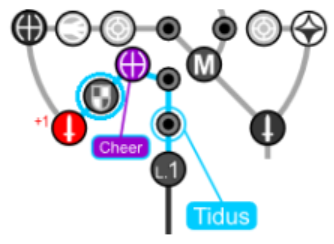
\includegraphics{graphics/tiduscheer}
	\end{itemize}
\end{spheregrid}
\begin{battle}[750]{Kimahri}
	\begin{itemize}
		\tidusf Attack x3-7, depending on crits/Strength node.
		\tidusf Each attack does average of 125, so 6 attacks averaging that will kill.
		\tidusf Need either Str Node, 2 Evades, 1 Crit, or +7 damage, otherwise Potion after 6th Attack
	\end{itemize}
\end{battle}
\begin{enumerate}[resume]
	\item \sd, continue running
\end{enumerate}
\begin{battle}{Garuda}
	\begin{itemize}
		\summon{\valefor}
		\valeforf Thunder x6 to build \od
	\end{itemize}
\end{battle}
\begin{enumerate}[resume]
	\item If you didn't do the sphere grid yet, do it now.
	\item \formation{\tidus}{\yuna}{\lulu}
\end{enumerate}
\begin{battle}{Garuda}
	\begin{itemize}
		\item Flee using the Escape Command
	\end{itemize}
\end{battle}
\begin{encounters}
	\begin{itemize}
		\item Dingo: \tidus\ Attack
		\item Condor: \wakka\ Attack
		\item Water Flan: \lulu\ Thunder
	\end{itemize}
\end{encounters}
\begin{enumerate}[resume]
	\item At Besaid Beach go onto the boat.
\end{enumerate}
	\chapter{S.S. Liki}

\begin{enumerate}
	\item \cs[2:00], walk up to \yuna, \sd, walk back to \wakka, \sd, walk back up to \yuna, \cs + 4 \skippablefmv[4:20], \sd\ from `Sin!'
\end{enumerate}
\begin{battle}[2000]{Sin Fin}
	\begin{itemize}
		\tidusf Defend
		\switch{\yuna}{\lulu}
		\luluf Thunder the Sin Fin
		\kimahrif Lancet the Sin Fin
		\enemyf Moves
		\tidusf Defend
		\kimahrif Lancet the Sin Fin
		\luluf Thunder the Sin Fin
		\switch{\tidus}{\yuna}
		\summon{\valefor}
		\valeforf Energy Blast \od\ on Sin Fin
	\end{itemize}
\end{battle}
\begin{enumerate}[resume]
	\item \fmv+\cs[1:40]
\end{enumerate}
\begin{battle}[2000]{Sinspawn Echuilles}
	\begin{itemize}
		\tidusf Cheer x2
		\wakkaf Dark Attack
		\tidusf Attack x2 \textit{if Str Node else} Cheer x2
		\wakkaf Attack x2
		\enemyf Blender
		\wakkaf Attack x2
		\tidusf Attack x2, one less if either \tidus\ crits or \wakka\ crits twice.
		\tidusf \od
	\end{itemize}
	Check for \textbf{Ice Brand, Ice Ball}
\end{battle}
\begin{enumerate}[resume]
	\item \skippablefmv+\cs[1:30], \sd\ during \tidus\ monologue.
\end{enumerate}
\newpage
	\chapter{Kilika}

\begin{enumerate}
	\item \sd\ on exiting the boat, go up and left, \sd. \skippablefmv[2:00], (press Start immediately after skip) \sd
	\item Exit inn, go right to \wakka, \sd. Go left and up to Kilika Woods, \sd
\end{enumerate}
\begin{battle}{Lancet Tutorial}
	\begin{itemize}
		\item \sd
		      \kimahrif Lancet
		      \switch{\kimahri}{\yuna}
		      \yunaf Defend
		      \tidusf Attack
		      \luluf Fire
	\end{itemize}
\end{battle}
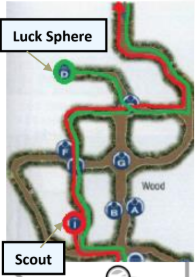
\includegraphics{graphics/kilikamap}
\begin{enumerate}[resume]
	\item Go left and up the hidden path, \pickup{Scout}
\end{enumerate}
\begin{spheregrid}
	\begin{itemize}
		\tidusf
		\begin{itemize}
			\item Move $\leftarrow\leftarrow$
			\item Flee, Agi+1
		\end{itemize}
	\end{itemize}
	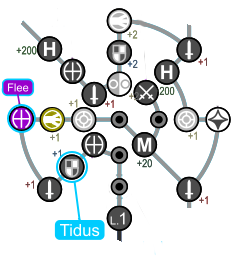
\includegraphics{graphics/Tidus_Kilika}
\end{spheregrid}
\begin{equip}
	\begin{itemize}
		\wakkaf Scout
		\item \textit{If you have them:}
		      \begin{itemize}
			      \wakkaf Ice Ball
			      \wakkaf Armguard
		      \end{itemize}
		\item \textit{If you got the Ice Brand:}
		      \begin{itemize}
			      \tidusf Ice Brand
		      \end{itemize}
	\end{itemize}
\end{equip}
\begin{enumerate}[resume]
	\item \formation{\tidus}{\yuna}{\wakka}
	\item Continue up the hidden path, following the map. Fill up \valefor\ \od\ with the first set, then do the rest of the encounters with the second set.
	\item Need 16 Speed Spheres from this point on. Need 45-55 AP on \tidus, which is about 5-7 kills.
\end{enumerate}
\bothvfill\winvfill\lossvfill
\begin{encounters}
	On Pre-Empts, Defend on Everyone.
	\begin{itemize}
		\item Killer Bee + Yellow Element:
		      \begin{itemize}
			      \tidusf Defend
			      \summon{\valefor}
			      \valeforf Boost
			      \valeforf Thunder Killer Bee
			      \valeforf Water Yellow Element
		      \end{itemize}
		\item Dinonix + Yellow Element
		      \begin{itemize}
			      \tidusf Attack Dinonix
			      \summon{\valefor}
			      \valeforf Boost x2
			      \valeforf Water Yellow Element
		      \end{itemize}
		\item Killer Bee + Dinonix + Yellow Element
		      \begin{itemize}
			      \tidusf Attack Dinonix
			      \summon{\valefor}
			      \valeforf Boost
			      \valeforf Thunder Killer Bee
			      \valeforf Water Yellow Element
		      \end{itemize}
		\item Killer Bee x2 + Ragora
		      \begin{itemize}
			      \tidusf Attack Ragora
			      \summon{\valefor}
			      \valeforf Thunder Killer Bee
			      \valeforf Thunder Killer Bee
			      \valeforf Fire x2 Ragora
		      \end{itemize}
		\item Ragora (Bad Encounter)
		      \begin{itemize}
			      \tidusf Defend
			      \summon{\valefor}
			      \valeforf Boost
			      \valeforf Sonic Wings
			      \valeforf Fire x2
		      \end{itemize}
		\item 2x Ragora (Super Bad Encounter)
		      \begin{itemize}
			      \tidusf Defend
			      \summon{\valefor}
			      \valeforf Boost
			      \valeforf Dismiss
			      \wakkaf Defend
			      \item Flee
		      \end{itemize}
	\end{itemize}
\end{encounters}
\begin{encounters}
	\begin{itemize}
		\item Killer Bee: \wakka Attack
		\item Dinonix: \tidus\ Attack
		      \yunaf Defend
		\item Ragora: Flee
		\item Flee whatever is left.
	\end{itemize}
\end{encounters}
\begin{enumerate}[resume]
	\item \sd
	\item \formation{\tidus}{\yuna}{\wakka}
	\item \save
\end{enumerate}
\bothvfill\winvfill\lossvfill
\begin{battle}[3000]{Sinspawn Geneaux}
	\begin{itemize}
		\item \textit{If \tidus\ is going before \yuna:}
		      \begin{itemize}
			      \tidusf Attack Main Body
			      \summon{\valefor}
			      \valeforf Energy Blast \od
			      \valeforf Fire x4-5
		      \end{itemize}
		\item \textit{Else:}
		      \begin{itemize}
			      \switch{\yuna}{\kimahri}
			      \kimahrif Attack Main Body
			      \tidusf Defend
			      \switch{anyone}{\yuna}
			      \summon{\valefor}
			      \valeforf Energy Blast \od
			      \valeforf Fire x4
		      \end{itemize}
	\end{itemize}
	Guaranteed 2 Power Spheres.
\end{battle}
\begin{enumerate}[resume]
	\item \sd\ on stone steps and temple. go into temple. Walk up to \wakka\ and Pray. \sd\ inside temple and go up steps. Wait for lift and \sd.
\end{enumerate}
\begin{trial}
	\begin{itemize}
		\item Take the sphere from the pedestal
		\item Place into the door, take it off of the door.
		\item Place sphere into the next door, take the sphere back.
		\item Place the sphere into the right holder
		\item Touch glpyh
		\item Take the sphere from the next room
		\item Place it into the left holder
		\item Take the glyph sphere from the pedestal
		\item Place it in the Fire Room
		\item Take the sphere that you put into the right holder
		\item Use it to open the door in the Fire Room
		\item Take the sphere off the door
		\item Enter the Fayth room
	\end{itemize}
\end{trial}
\begin{enumerate}[resume]
	\item In Fayth room, \sd, speak to \wakka\ first. Try to leave room, \sd, name \ifrit
	\item Hold down to exit temple, \cs[0:40], \sd
	\item Go south through Kilika Woods, take the left path and \pickup{Luck Sphere}, referencing map.
	\item Exit Kilika Woods same way that you entered, treating fights the same way as above.
	\item Go down and right to S.S. Winno. \sd
\end{enumerate}
	\chapter{S.S. Winno}
\begin{enumerate}
	\item \cs[1:10], exit door on the right. \sd\ with Oaka, then give him 1100 Gil. Run outside, go up to the top deck for \wakka\ and \lulu\ cutscene, \sd
	\item Run up the blitzball on the front of the boat. \cs[1:10]
	\item Follow the tutorial, fail the minigame
	\item \sd\ on \yuna's scene, do not save. \skippablefmv[0:30] if you buffered the Start command in Kilika.
\end{enumerate}
\vfill
\ 
\columnbreak
\ \newline
	\chapter{Luca}

\begin{enumerate}
  \item \sd, go right and up to the next screen, \cs[2:30]. Don't save.
  \item \sd\ in locker room. Don't do the tutorial. \sd, walk down, \sd
  \item Walk down to next screen, \sd. Whistle \cs[0:30], walk right to next screen.
  \item \sd, run to the cafe. \sd, \skippablefmv+\cs[1:20], \sd
  \item Run left to next screen, then left to the docks. Run north to the next screen.
\end{enumerate}
\vfill
\begin{battle}{Machina}
  \begin{itemize}
    \item \textit{For the first two encounters:}
          \begin{itemize}
            \tidusf Defend
            \kimahrif Defend
            \luluf Thunder
          \end{itemize}
    \item \textit{For the third encounter:}
          \begin{itemize}
            \item \textit{First Wave}
                  \begin{itemize}
                    \tidusf Attack
                    \kimahrif Attack
                    \luluf Thunder a different Machina
                    \tidusf Attack
                    \kimahrif \od\ Seed Cannon \textit{if no crits else} Attack
                  \end{itemize}
            \item \textit{Second Wave}
                  \begin{itemize}
                    \tidusf Defend
                    \kimahrif Defend
                    \luluf Thunder
                  \end{itemize}
            \item \textit{Third Wave}
                  \begin{itemize}
                    \tidusf Attack
                    \kimahrif Attack or \od\ Seed Canon
                    \luluf Thunder a different Machina
                  \end{itemize}
          \end{itemize}
  \end{itemize}
\end{battle}
\begin{enumerate}[resume]
  \item If anyone is Critical HP, use Potions.
  \item Run right. Do the below Sphere Grid if \tidus\ has 5 S.Levels.
\end{enumerate}
\begin{battle}[3000]{Oblitzerator}
 \begin{itemize}
    \kimahrif Defend
    \tidusf Defend \textit{If No Early Haste Else} Haste \lulu
    \luluf Thunder Crane x3
    \tidusf Use Crane after \lulu's string
    \kimahrif Defend
    \luluf Thunder
    \tidusf Attack
  \end{itemize}
  Check for \textbf{Lightning Steel, Thunder Ball}
\end{battle}
\begin{enumerate}[resume]
  \item \cs[2:00], \sd\ during and after Blitzball game.
\end{enumerate}
\begin{spheregrid}
  \begin{itemize}
    \tidusf (5 S.Lvl)
    \begin{itemize}
	    \item Move $\downarrow \searrow\searrow$
	    \item +1 Str, Haste, +20 MP
  \end{itemize}
  \end{itemize}
  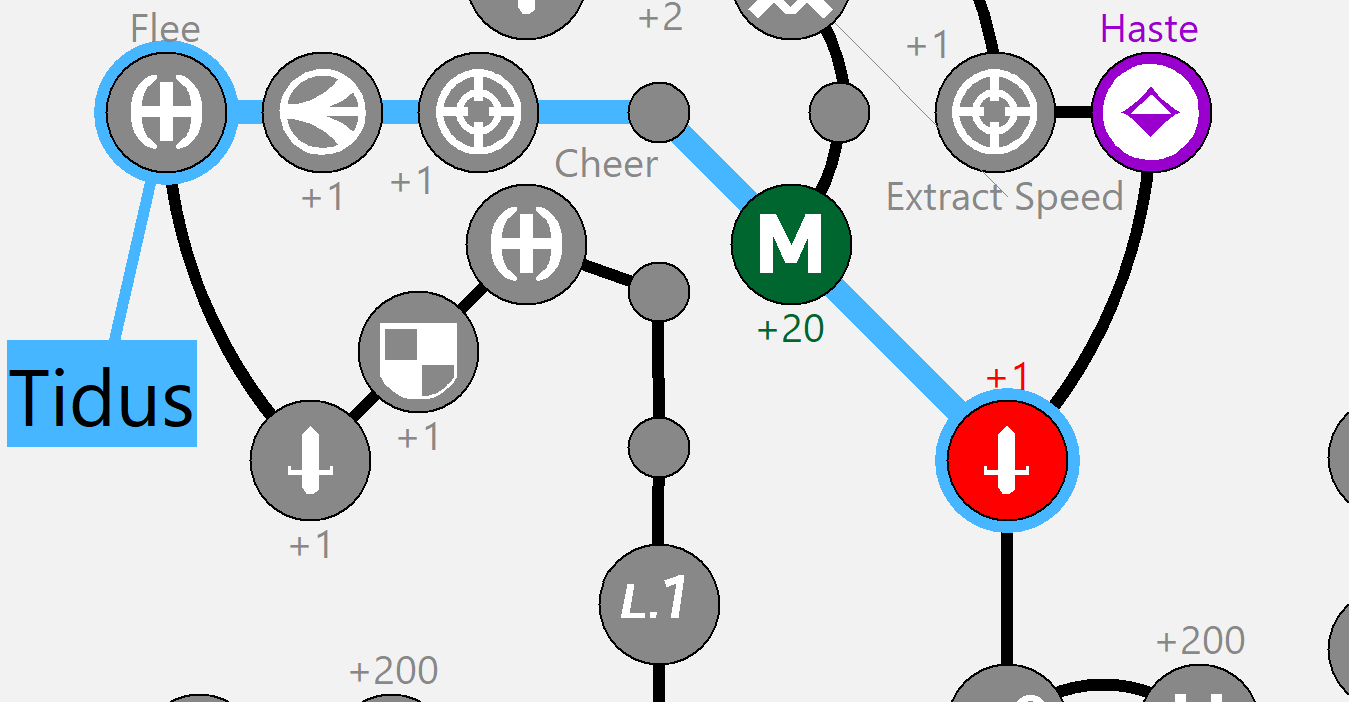
\includegraphics{graphics/haste}
\end{spheregrid}
\begin{enumerate}[resume]
  \item Auto-Sort items
  \end{enumerate}
\begin{equip}
  \begin{itemize}
    \item \textit{If you got Lightning Steel}
          \begin{itemize}
            \tidusf Lightning Steel
          \end{itemize}
   \item \textit{If you got Thunder Ball}
   		\begin{itemize}
   		\wakkaf Thunder Ball
   		\end{itemize}
  \end{itemize}
\end{equip}
\begin{enumerate}[resume]
  \item Run South for the next two screens. \save. Go up the stairs to the locker room, \sd
  \item Go back into locker room, speak to \wakka, \sd, \cs[1:20]. \sd\ after \lulu\ scene. \cs[1:40] on Auron Entrance.
\end{enumerate}
\begin{blitzball}
  \begin{itemize}
  \item \textbf{First Half:}
  \begin{itemize}
    \item \textit{If Luca wins the Blitzoff:}
          \begin{itemize}
            \item Triangle, switch the mode to \textbf{Mark Mode}, and then \textbf{Left Side}
            \item When Graav is close to your central player, return to \textbf{Normal Mode}
          \end{itemize}
    \item \textit{When you get the ball:}
          \begin{itemize}
            \item Change to \textbf{Manual A} and \textbf{Normal Mode}
            \item down some, pass the ball to \tidus
            \tidusf Swim next to Jassu, pass to Jassu
            \item Hide behind the Goalie
            \item If you aggroed a Goer, Swim Around
          \end{itemize}
          \end{itemize}
    \item \sd\ during half time
    \item \textbf{Second Half:}
    	\begin{itemize}
    \item \textit{If Luca wins the Blitzoff:}
          \begin{itemize}
            \item Triangle, switch the mode to \textbf{Mark Mode}, and then \textbf{Right Side}
            \item When Graav is close to your central player, return to \textbf{Normal Mode}
          \end{itemize}
    \item \textit{When you get the ball:}
    	\item Pass to Jassu if he doesn't have it
    	\item Swim to the Bottom Middle
    	\item Wait until 2:20, if Abus Aggros then Break
    	\item Swim to the Left, aggro Balgerda (bottom player), then swim back some
    	\item Pass to \tidus\ before Balgerda gets in range to block
    	\tidusf Swim close to the Goal and Sphere Sphot before anyone is close enough to block
    	\begin{itemize}
    		\item If 1 Defender and 2:49, Sphere Shot over the Defender
    		\item Otherwise, Break and Sphere Shot
    		\item If 2 Defenders, Break 1, Sphere Shot
	\end{itemize}
	\item \sd\ during \wakka\ \cs
	\item If you need to Score or it's 1-1, then do the same as above with Jassu
	\item Wait until 4:20 then aggro Balgerda, Pass to \wakka
	\wakkaf swim close and Venom Shot, or Break, Venom Shot
	\end{itemize}
  \item Don't try to score in the First Half
  \item If you're losing, Change to \textbf{Mark Mode} and lose the game.
  \end{itemize}
\end{blitzball}
\begin{enumerate}[resume]
  \item \sd, \cs[1:00], Don't Save
\end{enumerate}
\begin{battle}{Sahagin Chief}
  \begin{itemize}
    \item{If no Lightning Steel:}
          \begin{itemize}
            \tidusf Haste \tidus
            \wakkaf Attack one Sahagin for the first two waves, defend on the third wave
            \tidusf Attack the other Sahagin
            \wakkaf Potion if \tidus\ has less than 156 HP
          \end{itemize}
    \item{If Lightning Steel:}
          \begin{itemize}
            \tidusf Haste \tidus
            \tidusf Cheer x2
            \wakkaf Attack
            \tidusf Attack
          \end{itemize}
  \end{itemize}
Each Overkill is +1 Power Sphere
\end{battle}
\begin{enumerate}[resume]
  \item \sd, \skippablefmv. Overkill on Vouivre is +1 Power Sphere
\end{enumerate}
\begin{battle}[1800]{Garuda}
  \begin{itemize}
    \tidusf Haste \auron
    \auronf Attack x3
    \wakkaf Defend, Potion if \tidus\ is less than 312 HP
    \tidusf Attack
    \tidusf Defend
    \wakkaf Defend, Potion if \auron\ is less than 202 HP
    \auronf Attack x3
    \item Don't revive non-\auron\ party members
  \end{itemize}
Overkill is +1 Power Sphere
\end{battle}
\begin{enumerate}[resume]
  \item \cs+\skippablefmv[1:30]. Don't save. \sd\ the Auroch scene
  \item \cs[4:50]. Run north to the hidden chests, \pickup{Magic and HP Sphere}
  \item Run South and try to speak to \auron\ while he's walking away.
  \item Follow red arrow to \yuna. \sd\ during guardian scene. Walk to \yuna, \cs[4:20]
\end{enumerate}
	\chapter{Mi'ihen Highroad}

\begin{enumerate}
  \item Walk up. Forced encounter, \sd. Walk up, \sd\ during Maechen Scene.
\end{enumerate}
\begin{encounters}
  \begin{itemize}
    \item Bomb:
          \begin{itemize}
            \switch{anyone}{\kimahri}
            \kimahrif Lancet Bomb, learn \textbf{Self Destruct}
            \item Flee.
          \end{itemize}
    \item Else Flee,  Heal afterwards if it was an ambush.
  \end{itemize}
\end{encounters}
\begin{enumerate}[resume]
  \item {Mi'ihen Skip}
        \begin{itemize}
          \item After Maechen Scene, run up as quickly as possible.
          \item Go to the White Spot on the ground towards the left before the Man in Blue
          \item Speak to the man, get the \textbf{Hunter's Spear}
          \item Mash and step forward over the cutscene line
          \item Walk up during the cutscene to the next screen.
        \end{itemize}
  \item Make sure you get the \textbf{Hunter's Spear} if you fail the skip.
  \item Go right and \sd\ at Calli scene. Continue walking up. \sd\ Luzzu scene, \sd\ Shelinda scene
  \item \formation{\tidus}{\wakka}{\kimahri}
  \item Go to the next screen
  \item Go to the Al-Bhed shop, \sd. Walk out of the shop and \cs[5:30]
  \item Leave shop, \sd. \sd\ on Rin. Walk outside.
\end{enumerate}
\begin{battle}{Chocobo Eater}
  \begin{itemize}
    \tidusf Haste Boss
    \item Defend with everyone.
    \item Swap any characters that fall into crit HP with someone in the back.
  \end{itemize}
\end{battle}
\begin{enumerate}[resume]
  \item \sd
  \item Walk north, \save. Walk north to next screen. Walk to blocked road, \sd. Speak to the guard on the right, \sd, walk back, \sd. Walk up to next screen.
\end{enumerate}
	\chapter{Mushroom Rock Road}

\begin{enumerate}
	\item \sd, \cs.
	\item Clasko Skip
	      \begin{itemize}
		      \item Run forward to the 3 Soldiers
		      \item Wedge yourself behind the right soldier by holding Left for a second
		      \item Tap Down-Right, X to speak to the bottom soldier
		      \item If the Soldier got away:
		            \begin{itemize}
			            \item Run up near the white spot on the wall near the trigger
			            \item Talk to the Soldier right after he pushes you into the trigger
			            \item Mash until trigger dialogue during the \cs
		            \end{itemize}
	      \end{itemize}
	\item Flee from any encounters, go to the next screen.
	\item \save. Go up the lift. Follow path.
	\item \formation{\tidus}{\wakka}{\auron}
\end{enumerate}
\begin{battle}{Non-Garuda Non-Ambush Anything}
	Try to make it an encounter with a Funguar, but take whatever the third encounter is.
	\begin{itemize}
		\switch{\tidus}{\kimahri}
		\kimahrif Defend
		\wakkaf Defend
		\switch{\auron}{\yuna}
		\summon{\valefor}
		\valeforf Energy Ray
	\end{itemize}
\end{battle}
\begin{equip}
	\begin{itemize}
		\wakkaf Scout/Ice Ball
	\end{itemize}
\end{equip}
\begin{enumerate}[resume]
	\item \formation{\tidus}{\wakka}{\auron}
\end{enumerate}
\vfill
\begin{spheregrid}
	\begin{itemize}
		\yunaf (8 S.Lvl)
		\begin{itemize}
			\item Use Magic Sphere
			\item +4 Magic
			\item Move $\rightarrow\rightarrow\rightarrow\rightarrow$
			\item +3 MagDef, +3 Magic, +20 MP
		\end{itemize}
		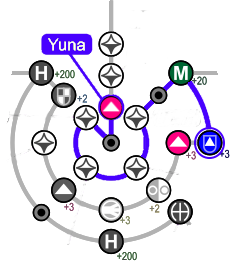
\includegraphics{graphics/Yuna_MRR_1}
		\kimahrif (6 S.Lvl)
		\begin{itemize}
			\item Move $\rightarrow$
			\item +200 HP
			\item Move $\leftarrow\uparrow$
			\item +200 HP
			\item Move $\leftarrow$
			\item +200 HP
		\end{itemize}
		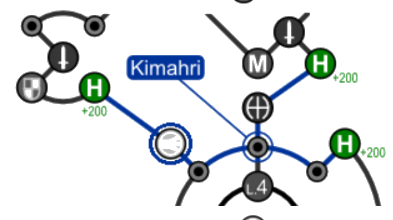
\includegraphics{graphics/kimahrimmr}
		\wakkaf (7 S.Lvl)
		\begin{itemize}
			\item Move $\rightarrow x4 (\downarrow)$Silence Attack
			\item +2 Strength
		\end{itemize}
		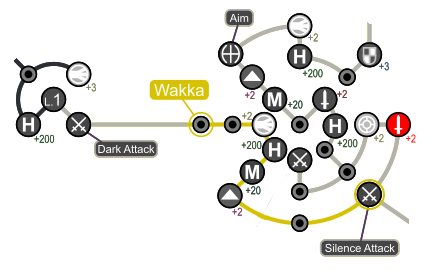
\includegraphics[width=.9\columnwidth]{graphics/Wakka_Grid}
	\end{itemize}
\end{spheregrid}
\vfill
\begin{encounters}
	The actions that you do here to charge \valefor's overdrive will change depending on the enemies. Follow the flow chart.
	\begin{itemize}
		\item \textit{If the enemy is a Garuda:}
		\begin{itemize}
			\item Flee
		\end{itemize}
		\item \textit{If there is a Lamashtu, a Gandarewa and no Raptor, or you didn't get a Funguar \od\ in the previous fight}:
		\begin{itemize}
			\switch{\tidus}{\kimahri}
		\end{itemize}
		\item \textit{If there is a Lamashtu:}
		\begin{itemize}
			\kimahrif Attack Lamashtu
		\end{itemize}
		\item \textit{Otherwise:}
		\begin{itemize}
			\item \kimahri\ or \tidus: Defend
		\end{itemize}
		\item \textit{If there is a Raptor:}
		\begin{itemize}
			\wakkaf Attack Raptor
		\end{itemize}
		\item \textit{If there is a Gandarewa and no Raptor:}
		\begin{itemize}
			\kimahrif Lancet Gandarewa \textit{If you didn't attack a Lamashtu}
			\wakkaf Attack Gandarewa
			\item \textit{If the Gandarewa is still alive:} Flee
		\end{itemize}
		\switch{\auron}{\yuna}
		\summon{\valefor}
		\item \textit{If there is still a Gandarewa:}
		\begin{itemize}
			\valeforf Water Gandarewa
		\end{itemize}
		\item \textit{Otherwise, if there is a Lamashtu or a Funguar}
		\begin{itemize}
			\valeforf Fire the Lamashtu or the Funguar
		\end{itemize}
		\valeforf Boost
		\valeforf Blizzard Red Element
	\end{itemize}
\end{encounters}
\begin{enumerate}[resume]
	\item Keep the \formation{\kimahri}{\wakka}{\yuna}
	\item Keep on fighting encounters until Yuna can do the next Sphere Grid menu, which is at 3 S. Levels, as you progress through the area.
\end{enumerate}
\begin{encounters}
	\begin{itemize}
		\wakkaf Attack Raptors or Gandarewas
		\yunaf Defend
		\item Flee
	\end{itemize}
\end{encounters}
\begin{spheregrid}
	\begin{itemize}
		\yunaf (3 S.Lvl)
		\begin{itemize}
			\item Move $\downarrow\downarrow$
			\item +3 Magic, +3 Agi
		\end{itemize}
		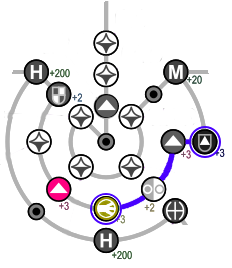
\includegraphics{graphics/Yuna_MRR_2}
	\end{itemize}
\end{spheregrid}
\begin{enumerate}[resume]
	\item After the Sphere Grid, \formation{\tidus}{\yuna}{\wakka}, and you can stop grinding encounters.
	\item Speak to the man to the left, right before the elevator that brings you up the to HQ Elevator, on the second screen, for 400 Gil. Go on lift, go to HQ.
	\item Walk down and \sd. Walk right to next screen, then right, \sd. Walk right to O'aka
\end{enumerate}
\begin{shop}{10890}
	\begin{itemize}
		\item Sell
		      \begin{itemize}
			      \item Hi-Potions
			      \item X-Potions
			      \item Elixirs
			      \item Hunter's Spear
			      \item Anything other than Longsword, Official Ball, Lightning Steel, Thunder Ball
		      \end{itemize}
		\item Buy
		      \begin{itemize}
			      \item Sentry, Equip
		      \end{itemize}
	\end{itemize}
\end{shop}
\begin{enumerate}[resume]
	\item \save
	\item \sd, go right, \cs[1:00], \sd\ after Seymour. Go down to guard, use the \nth{2} option to confirm Yes, \sd
\end{enumerate}
\begin{battle}[12000]{Sinspawn Gui 1}
	\begin{itemize}
		\switch{\yuna}{\auron}
		\auronf Power Break Main Body
		\tidusf Defend
		\wakkaf Switch Weapon to Thunder Ball, Power Ball, or Official Ball
		\switch{\wakka}{\kimahri}
		\kimahrif Self Destruct main body
		\switch{\tidus}{\yuna}
		\summon{\valefor}
		\valeforf Energy Blast \od\ x2
		\item \textit{If \valefor\ doesn't charge second \od:}
		      \begin{itemize}
			      \valeforf Shield until Gui used a physical attack
			      \valeforf Boost
			      \valeforf Energy Blast \od
		      \end{itemize}
		\item \textit{If Self Destruct Crit \textit{(7464)}:}
		      \begin{itemize}
			      \valeforf Energy Blast
			      \valeforf Thunder Main Body
		      \end{itemize}
		\item \textit{If Power Break Failed}
		      \begin{itemize}
			      \valeforf Energy Blast
			      \summon{\ifrit} once \valefor\ dies.
			      \ifritf Fire Main Body until 3000 HP
			      \ifritf Hellfire
		      \end{itemize}
	\end{itemize}
\end{battle}
\begin{enumerate}[resume]
	\item \cs+\skippablefmv[2:20]. \sd\ Seymour dialogue.
\end{enumerate}
\begin{battle}[6000]{Sinspawn Gui 2}
	\begin{itemize}
		\item \textit{If \yuna\ or \valefor\ don't have \od:}
		      \begin{itemize}
			      \item \textbf{\textcolor{YellowGreen}{Seymour}}: Thundara Head ($\leftarrow$)
			      \item \textbf{\textcolor{YellowGreen}{Seymour}}: Thundara Body x5
			            \yunaf Defend
			            \auronf Defend
		      \end{itemize}
		\item \textit{If they do:}
		      \begin{itemize}
			      \item \textbf{\textcolor{YellowGreen}{Seymour}}: Thundara Body x2
			            \summon{\valefor} or Grand Summon \valefor
			            \valeforf Energy Blast
		      \end{itemize}
	\end{itemize}
\end{battle}
\begin{enumerate}[resume]
	\item \sd, \cs+\skippablefmv[2:00] (press Start immediately after the skip. Do not use it on the upcoming scenes, as you will crash your game). Walk left and up to Gatta, \sd. \fmv+\cs[1:30], \sd\ during \tidus\ monologue. \cs[1:00], \sd
	\item Walk left, \sd. Walk left, speak to \auron, \sd. \save\ if \auron\ is in critical HP. Go up and right, \sd, exit area, \sd.
\end{enumerate}


	\chapter{Djose}

\begin{spheregrid}
	\begin{itemize}
		\tidusf
		\begin{itemize}
			\item Move $\rightarrow\uparrow$
			\item Str+1, HP+200, Agil+2
		\end{itemize}
		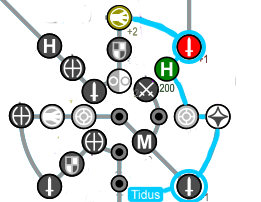
\includegraphics[width=.6\columnwidth]{graphics/Tidus_post_gui}
		\wakkaf
		\begin{itemize}
			\item Move $\uparrow\uparrow\uparrow$ (PC) or $\uparrow\uparrow$ (PS2)
			\item Str +2
		\end{itemize}
		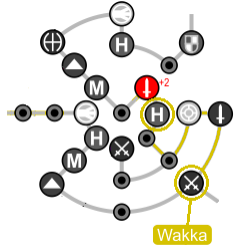
\includegraphics[width=.6\columnwidth]{graphics/djosewakka}
	\end{itemize}
\end{spheregrid}
\begin{enumerate}
	\item \formation{\tidus}{\yuna}{\auron}
	\item Walk North.
\end{enumerate}
\begin{encounters}
	\begin{itemize}
		\item Basilisk:
		      \begin{itemize}
			      \switch{anyone}{\kimahri}
			      \kimahrif Lancet Basilisk, learn \textbf{Stone Breath}
			      \item Flee.
		      \end{itemize}
		\item Else Flee
	\end{itemize}
\end{encounters}
\begin{enumerate}[resume]
	\item Continue walking north, \sd, walk up to the next screen.
	\item Walk along bridge to next screen, \sd, walk into temple. Speak to \auron\ at the doorway, \sd, walk up the stairs.
\end{enumerate}
\vfill
\begin{trial}
	\begin{itemize}
		\item Take the sphere from the left wall
		\item Place into door
		\item Take the sphere from the right wall
		\item Place into door
		\item Take the sphere from the left wall
		\item Push pedestal to the right
		\item Put sphere into the far right wall
		\item Take right sphere
		\item Place into the far right wall
		\item \cs
		\item Take sphere from far right wall
		\item Reset puzzle with the far left tile
		\item Place sphere into pedestal
		\item Take the pedestal sphere
		\item Put sphere into right wall
		\item Take the far right sphere
		\item Put into pedestal
		\item Push pedestal through the door
		\item Jump onto pedestal
		\item Push the second pedestal, return to main room
		\item Take the charged sphere from the right wall
		\item Place charged sphere into the left wall
		\item Reset
		\item Place the two pedestal spheres in the first left and right walls
		\item Go onto the lift in the center
		\item Push all the pedestals in, walk up the stairs
	\end{itemize}
\end{trial}
\begin{enumerate}[resume]
	\item Talk to \auron, wait. \sd, try to leave, \sd, name \ixilon
	\item Speak to \auron, enter the temple and go to the left room. Open the chest for a \textbf{Remedy}. Speak to the priest, \sd. Exit the temple, \sd
	\item Go left, \pickup{4000 Gil}, cross the bridge, \sd, exit, \sd, go up to Moonflow.
\end{enumerate}
	\chapter{Moonflow}

\begin{enumerate}
  \item Walk north, \sd\ on Kimahri Scene.
  \item Near the end of the screen, go left through the hidden path. \pickup{Magic Def Sphere}.
  \item Walk north, \sd, walk left, \sd, walk left past 2 screens, \sd.  Potion/Cure \tidus\ if he got injured.Walk right and ride ze shoopuf, \sd.
\end{enumerate}
\begin{battle}[4000]{Extractor}
  \begin{itemize}
    \tidusf Haste self, then \wakka
    \wakkaf Attack
    \tidusf \textit{If Lightning Steel:}
    \begin{itemize}
      \item Cheer x1
    \end{itemize}
    \textit{Else:}
    \begin{itemize}
      \item Cheer x4
    \end{itemize}
    \tidusf Attack
    \textit{If got a Crit and don't have Thunder Ball:}
    \begin{itemize}
    	\wakkaf \od Thunder Reels before Extractor's 4th turn.
	\end{itemize}
  \end{itemize}
\end{battle}
\begin{enumerate}[resume]
  \item \sd, walk left to next screen, walk left and talk to \rikku, \sd
  \item Walk up to the forced encounter
\end{enumerate}
\begin{battle}{Rikku Tutorial}
  \begin{itemize}
    \item Complete tutorial
    \item \textit{If you have less than 23 Power Spheres:}
          \begin{itemize}
            \rikkuf \od\ Two Ability Spheres
          \end{itemize}
    \item \textit{Else:}
          \begin{itemize}
            \rikkuf \od\ Two Potions
          \end{itemize}
    \item Flee
  \end{itemize}
\end{battle}
\begin{enumerate}[resume]
  \item Walk to next screen.
  \item \formation{\tidus}{\wakka}{\auron}
  \item Heal everyone with Potions
  \item Walk north to next screen.
\end{enumerate}
	\chapter{Guadosalam}

\begin{enumerate}
	\item \sd, walk to Seymour's house, try to leave. Walk into room, speak to \auron, \sd, speak to \wakka, \lulu, \rikku, \yuna. \sd, \skippablefmv+\cs[5:50] if you buffered the Start command after Gui.
	\item Exit the house, walk down, \sd. Go to the Farplane. Hidden to the left in the screen going to the Farplane, \pickup{Lightning Marble x8}
	\item \sd, speak to \auron, go into the Farplane. \cs[1:20]. Speak to \wakka, \sd, speak to \yuna, \cs[2:10], \sd.
	\item Go to Seymour House Entrance, \sd
	\bothcb \wincb \losscb
	\item Guadosalam Skip:
	      \begin{itemize}
		      \item Stand outside of the Potion Shop
		      \item Wait until you get pushed by the Guado to trigger the skip
		      \item Run to the exit using the minimap
		      \item If on HD Remaster, speak to the woman on the left to stop her walking abit, then speak to the running Guado as the woman pushes you to into the door.
	      \end{itemize}
	      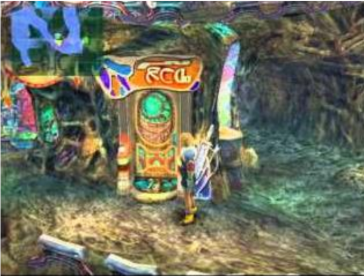
\includegraphics{graphics/guadoskipstandard}

	      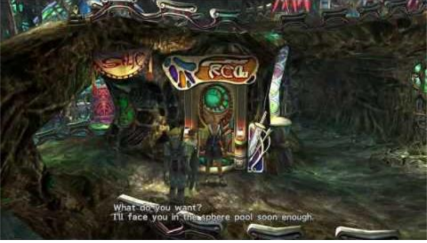
\includegraphics{graphics/guadoskipremaster}
\end{enumerate}
	\chapter{Thunder Plains}

\begin{enumerate}
	\item Walk north, dodging lightning. Try to end Thunder Plains with the Light Curtain. Flee all encounters
\end{enumerate}
\begin{enumerate}[resume]
	\item \sd\ when approaching Al Bhed shop. Walk into the shop when \rikku\ begs to go inside.
\end{enumerate}
\begin{shop}{2850-3450}
	\begin{itemize}
		\item Sell: Longsword, Katana
		\item \textit{\blitzloss:}
		      \begin{itemize}
			      \item Sell: Other Equipment worth 1k+ Gil
			      \item Buy: Baroque Sword (Do Not Equip)
		      \end{itemize}
		\item Buy:
		      \begin{itemize}
			      \item Shimmering Blade (Do Not Equip)
			      \item 3 Phoenix Downs
			      \item 3 Grenades, +1 for every Buer encounter you want for Speed Spheres, +1 if \blitzloss
		      \end{itemize}
	\end{itemize}
	Try to leave the shop with 7075 Gil
\end{shop}
\begin{enumerate}[resume]
	\item Walk into shop corridor, \cs[2:00]
	\item Speak to \auron, then to \rikku, \sd.
	\item Pickup the \textbf{Yellow Shield} outside the shop on the ground.
\end{enumerate}

\begin{encounters}
	\begin{itemize}
		\item Buer: If short on Speed Spheres, can throw Grenades
		\item Iron Giant:
		      \begin{itemize}
			      \switch{\tidus}{\rikku}
			      \rikkuf Steal Light Curtain
			      \switch{\wakka}{\tidus}
			      \tidusf Defend
			      \enemyf Attacks \rikku
			      \auronf Defend
			      \item Flee
		      \end{itemize}
		\item Larva: If \blitzloss, try to steal Lunar Curtain
		\item Melusine: Steal Petrify Grenade if want to.
	\end{itemize}
\end{encounters}
\begin{enumerate}[resume]
	\item Exit screen, go north, near the exit \sd, \cs[3:10]
\end{enumerate}
	\chapter{Macalania Woods}

\begin{enumerate}
	\item \sd, walk north, \sd, \save
	\item \formation{\tidus}{\rikku}{\auron}
	\item Follow path, \pickup{2000 Gil}
	\item Make sure that you build up \rikku\ \od, and that you do at least one of each of the following steals.
\end{enumerate}
\begin{encounters}
\begin{itemize}
	\item Chimera: Steal Arctic Wind, Flee
	\item Blue Elementa: Steal Fish Scale x2, Flee
	\item Else: Flee
\end{itemize}
\end{encounters}
\begin{enumerate}[resume]
	\item Follow path, \sd\ twice
	\item Catch butterfly near the exit to avoid encounters
	\formation{\tidus}{\yuna}{\kimahri}
	\item \save, talk to Oaka. Say his ``Prices are too expensive'', go in again.
\end{enumerate}
\begin{shop}{9075}
\begin{itemize}
	\item Buy: Sonic Steel, Equip
\end{itemize}
\end{shop}
\begin{enumerate}[resume]
	\item Run up, \sd. Enter the hidden path, walk to \auron, \sd
\end{enumerate}
\begin{battle}[12000]{Spherimorph}
\begin{itemize}
	\tidusf Change Armor to Yellow Shield
	\tidusf Defend
	\switch{\tidus}{\rikku}
	\rikkuf Grenade, check the Element
	\kimahrif Defend
	\yunaf Defend
	\rikkuf \od, Mag Def Sphere with
	\begin{itemize}
		\item Fire: Arctic Wind
		\item Ice: Bomb Core
		\item Water: Lightning Marble
		\item Thunder: Fish Scale
	\end{itemize}
\end{itemize}
\end{battle}
\begin{enumerate}[resume]
	\item \cs[1:50], \sd, \sd
	\item Auto Sort Items, put Phoenix Downs in the First Slot and Lightning Marbles in the Third
\end{enumerate}
\end{multicols}
\newpage
\begin{multicols}{2}
\begin{spheregrid}
\begin{itemize}
	\rikkuf
	\begin{itemize}
		\item Move down 2 nodes (1 if you're doing quick hit)
		\item Agi+3
	\end{itemize}
	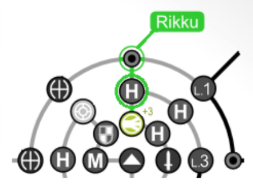
\includegraphics{graphics/macalaniarikku}
	\kimahrif
	\begin{itemize}
		\item Move to the bottom left of the grid
		\item Agi+3, Level 1 Key Sphere
		\item Move further left
		\item Level 1 Key Sphere
		\item Go to Steal Node
		\item Steal, Use
	\end{itemize}
	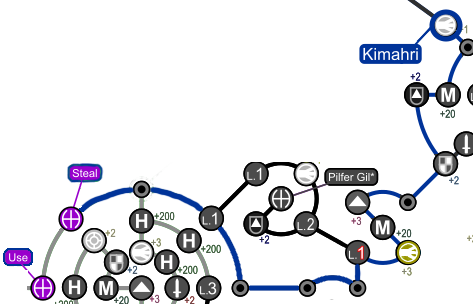
\includegraphics[width=.8\columnwidth]{graphics/Kimahri_post_spheremorph}
	\yunaf
	\begin{itemize}
		\item Agi +3, HP +200, Def +2
		\item Level 2 Key Sphere
		\item Str + HP Nodes
		\item Agi+2 Node
		\item Stop at Str +4
	\end{itemize}
	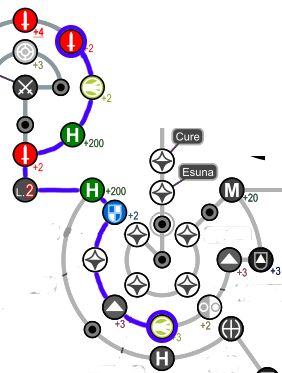
\includegraphics[width=.6\columnwidth]{graphics/Yuna_post_spheremorph}
\end{itemize}
\end{spheregrid}
\begin{enumerate}[resume]
	\item Heal Party, with Cure/Mega-Potions
	\item \formation{\tidus}{\lulu}{\kimahri}
	\item Talk to \auron\ on the way out, then exit
\end{enumerate}
\vfill

	\chapter{Lake Macalania}

\begin{enumerate}
	\item Run up and \sd
\end{enumerate}
\begin{battle}[16000]{Crawler}
	\begin{itemize}
		\switch{\tidus}{\rikku}
		\rikkuf Lightning Marble x1/2 Negator (1\,000 HP)
		\rikkuf Lightning Marble Crawler
		\kimahrif Lightning Marble Crawler
		\luluf Phoenix Down \rikku
		\ifthenelse{%
		\equal{\blitzresult}{win}}{%
			      \switch{\kimahri}{\yuna} \textit{If \kimahri\ didn't die}
			      \yunaf Defend
			      \rikkuf Lightning Marble Crawler
			      \luluf Phoenix Down \rikku\ \textit{If \kimahri\ didn't die else} Swap for \yuna\ and \yuna\ Phoenix Down \rikku
		}{\ifthenelse{\equal{\blitzresult}{loss}}{%
		\item \textit{If you have a Lunar Curtain:}
		      \begin{itemize}
			      \switch{\kimahri}{\yuna} \textit{If \kimahri\ didn't die}
			      \yunaf Defend
			      \rikkuf Lightning Marble Crawler
			      \luluf Phoenix Down \rikku\ \textit{If \kimahri\ didn't die else} Swap for \yuna\ and \yuna\ Phoenix Down \rikku
		      \end{itemize}
		      \item \textit{If you don't have a Lunar Curtain:}
		      \begin{itemize}
			      \kimahrif Steal
			      \rikkuf Lightning Marble Crawler
			      \switch{\lulu}{\yuna}
			      \yunaf Phoenix Down \rikku
		      \end{itemize}
		}{\ifthenelse{\equal{\blitzresult}{both}}{%
		\item \textit{If \blitzwin\ or you have a Lunar Curtain:}
		      \begin{itemize}
			      \switch{\kimahri}{\yuna} \textit{If \kimahri\ didn't die}
			      \yunaf Defend
			      \rikkuf Lightning Marble Crawler
			      \luluf Phoenix Down \rikku\ \textit{If \kimahri\ didn't die else} Swap for \yuna\ and \yuna\ Phoenix Down \rikku
		      \end{itemize}
		      \item \textit{If \blitzloss\ and don't have a Lunar Curtain:}
		      \begin{itemize}
			      \kimahrif Steal
			      \rikkuf Lightning Marble Crawler
			      \switch{\lulu}{\yuna}
			      \yunaf Phoenix Down \rikku
		      \end{itemize}
		}{}}}
		
		      \switch{\yuna}{\tidus}
		      \tidusf Defend
		      \rikkuf \od\ HP Sphere and Lightning Marble
	\end{itemize}
	\tidus, \yuna, \lulu\ need AP.
\end{battle}
\bothvfill
\winvfill
\lossvfill
\begin{spheregrid}
	\begin{itemize}
		\tidusf (22 S.Lvl)
		\begin{itemize}
			\item Level 2 Key Sphere
			\item Move $\rightarrow\uparrow$
			\item Str +4
			\item Move $\uparrow\uparrow$
			\item HP+200
			\item Move $\rightarrow\rightarrow\uparrow$
			\item HP+200, Str+4, Agi+2
			\blitzballdetermination[true]{%
				      \item Move $\rightarrow$
				      \item Use Strength Sphere, Activate it
				      \item Move $\uparrow\leftarrow\leftarrow$ or $\nwarrow\nwarrow$
			}{%
				      \item Move $\uparrow\nwarrow$			
			}
			\item HP+200, Str+4, Agi+2
			\item Move $\leftarrow$
			\item Str+4
		\end{itemize}
		\ifthenelse{\equal{\colstyle}{multi}}{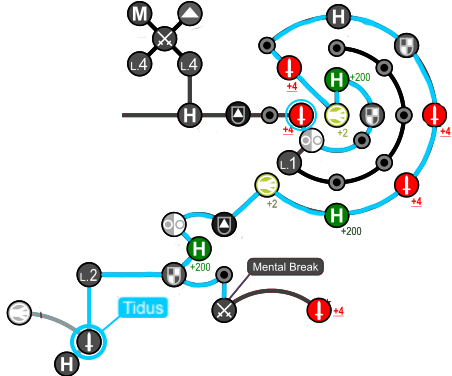
\includegraphics[width=.8\columnwidth]{graphics/Tidus_post_crawler}}{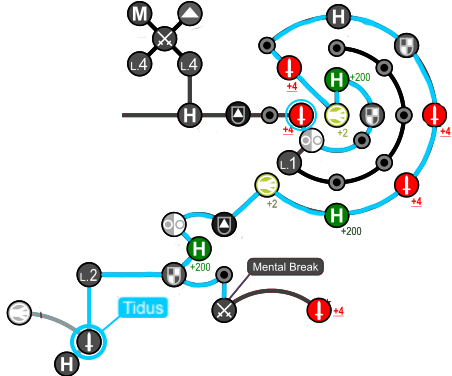
\includegraphics[width=.5\columnwidth]{graphics/Tidus_post_crawler}}
	\end{itemize}
\end{spheregrid}
\begin{enumerate}[resume]
	\item \sd, \cs[0:40], head to next screen
	\item Head to Temple, \sd. \save.
	\wincb
	\item Jyscal Skip (Ignore if playing with Cutscene Remover):
	      \begin{itemize}
		      \item Speak to Tromell for \textbf{Shell Targe}
		      \item Walk into the wall to the right of Tromell
		      \item Move slightly to the right, turn around and Talk to Tromell while moving Right.
		      \item If successful, walk forward while mashing Shelinda's dialogue.
		      \item When dialogue finishes, walk up the stairs, push the man, and go through.
		      \item If Shelinda is not saying her dialogue, talk to one of the musicians
	      \end{itemize}
	\item \sd, walk to Fayth room, \cs[2:10]
\end{enumerate}
\bothvfill
\begin{battle}[3000]{Seymour}
	\begin{itemize}
		\blitzballdetermination[true]{%
			\tidusf Switch Weapon to Brotherhood
			\tidusf Haste \tidus
			\enemyf Seymour Blizzara
			\tidusf Talk to Seymour
			\yunaf Change Weapon to Staff
			\enemyf Guado Guardians Blizzard/Thunder/Shremedy or do nothing
			\kimahrif Use Remedy on Confused character/Phoenix Down \yuna/Defend
			\switch{\yuna}{\auron}
			\auronf Defend
			\tidusf \od\ Spiral Cut Seymour
		}{%
			\tidusf Haste \tidus
			\tidusf Cheer
			\tidusf Talk to Seymour
			\yunaf Change Weapon to Staff
			\switch{\kimahri}{\rikku}
			\rikkuf Use Remedy on Confused character/Phoenix Down \yuna/Defend
			\switch{\yuna}{\kimahri}
			\kimahrif Use Remedy or Attack Confused character/Phoenix Down \yuna/Defend
			\tidusf Switch to Brotherhood
			\tidusf \od\ Spiral Cut Seymour
		}
	\end{itemize}
\end{battle}
\bothvfill
\lossvfill
\begin{battle}[18000]{Anima}
	\begin{itemize}
		\blitzballdetermination[true]{%
			\switch{\tidus}{\wakka}
			\wakkaf Change Weapon to anything
			\kimahrif Steal
			\enemyf Pain
			\switch{first survivor}{\tidus}
			\tidusf Attack x4
			\switch{second survivor}{\rikku}
			\rikkuf Phoenix Down \yuna/Steal
		}{%
			\rikkuf Use Lightning Marble/Arctic Wind
			\switch{\tidus}{\wakka}
			\wakkaf Change Weapon to anything
			\kimahrif Use Lightning Marble/Arctic Wind
			\enemyf Pain
			\switch{\wakka}{\tidus}, if \wakka\ died then switch \rikku\ instead.
			\tidusf Attack x4
			\switch{\kimahri}{\rikku} \textit{if you had to switch out \rikku\ before}
			\rikkuf Phoenix Down \yuna/Steal
		}
		\item \textit{If Tidus Misses:}
			\begin{itemize}
				\item On Tidus' 4th turn switch him for anyone but \yuna
				\item That character: Phoenix Down dead character
				\enemyf Pain
				\switch{first survivor}{\tidus}
				\item Continue the fight like normal
			\end{itemize}
	\end{itemize}
\end{battle}
\begin{battle}[6000]{Seymour}
	\begin{itemize}
		\tidusf Defend x2 until Multi-Thundara, Phoenix Down \rikku\ if she died before Multi-Thundara.
		\rikkuf Defend
		\tidusf Attack x2
	\end{itemize}
	\tidus\ and \yuna\ need AP.
\end{battle}
\begin{enumerate}[resume]
	\item Name \shiva
\end{enumerate}
\begin{spheregrid}
	\begin{itemize}
		\tidusf
		\begin{itemize}
			\item Move $\leftarrow\leftarrow\leftarrow\leftarrow$
			\item HP+200, Str+4
			\item Move $\leftarrow$
			\item Agi+2
		\end{itemize}
		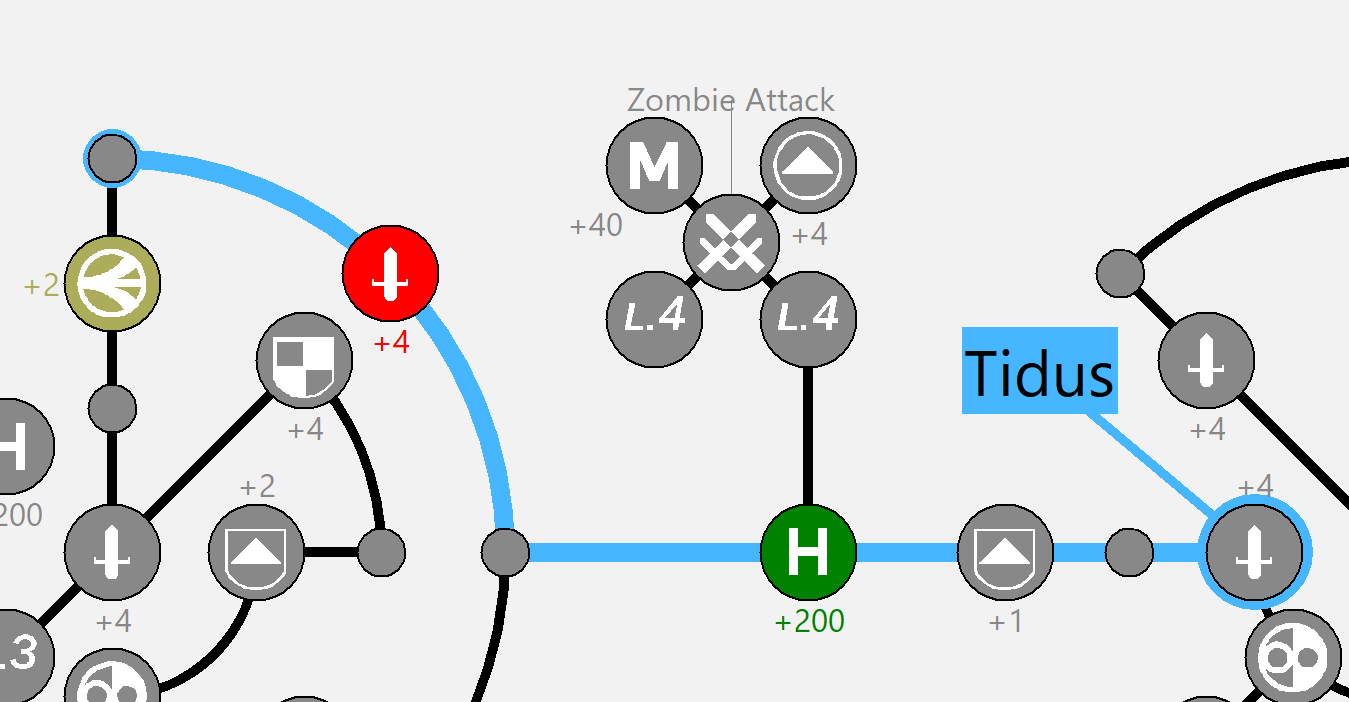
\includegraphics[width=.8\columnwidth]{graphics/Tidus_Post_Seymour}
	\end{itemize}
\end{spheregrid}
\winvfill
\begin{equip}
	\begin{itemize}
		\tidusf Sonic Steel
	\end{itemize}
\end{equip}
\begin{enumerate}[resume]
	\item \formation{\rikku}{\tidus}{\yuna}
	\item \save, exit Fayth room.
\end{enumerate}
\begin{trial}
	\begin{itemize}
		\item Slide pedestal to the right
		\item Take sphere from the right wall, place into pedestal
		\item Push pedestal up
		\item Take Glyph sphere from middle pillar
		\item Go downstairs and push pedestal to the right
		\item Place Glyph sphere in far left slot in the wall
		\item Go upstairs, pick up new sphere
		\item Go downstairs, place sphere in pillar
		\item Go upstairs, take the sphere at the top of the slope
		\item Place in last pillar
	\end{itemize}
\end{trial}
\begin{enumerate}[resume]
	\item Go to temple entrance, \sd
	\item Move south and go down the left path.
	\blitzballdetermination[true]{
		\item Try to not get caught by the Guados chasing you, if you get caught Flee
	}{
		\item Intentionally get caught by a Guado, kill the enemies to gain AP on Tidus
		\begin{encounters}
			\begin{itemize}
				\tidusf Attack Guado, then Surviving Enemies
				\rikkuf Silence Grenade
				\yunaf Defend
			\end{itemize}
		\end{encounters}
	}
\end{enumerate}
\blitzballdetermination{}{
\begin{spheregrid}
	\begin{itemize}
		\tidusf Move $\downarrow$
		\item Str+4
	\end{itemize}
	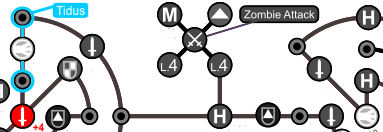
\includegraphics[width=.8\columnwidth]{graphics/tidus_bikanel}
\end{spheregrid}}
\winvfill
\bothvfill
\begin{battle}[18000]{Wendigo}
	\begin{itemize}
		\tidusf Haste \tidus
		\tidusf Switch Weapon to Brotherhood
		\tidusf Attack Guado B (Top One)
		\item \textit{If Light Curtain:}
			\begin{itemize}
				\rikkuf Light Curtain \tidus
			\end{itemize}
		\textit{Else:}
			\begin{itemize}
				\switch{\rikku}{\auron}
				\auronf Power Break
			\end{itemize}
		\tidusf Attack Wendigo until its dead, then Guado
		\yunaf Elixir \tidus/Phoenix Down dead character/Defend
		\switch{\yuna}{\lulu} on \yuna's 2nd turn
		\rikkuf Elixir \tidus/Phoenix Down dead character/Steal from the Guado/Defend
		\luluf Elixir \tidus/Phoenix Down dead character/Defend
	\end{itemize}
	\yuna, \tidus\ need AP. Helpful if \lulu\ gets it.
	Guaranteed 2 Power Spheres.
\end{battle}
\begin{enumerate}[resume]
	\item Run up to \rikku, \sd, walk up to \yuna, \sd, \save, run past \kimahri\ and go to the hidden area to \pickup{Level 2 Key Sphere}
	\winvfill
	\item Run up to \auron\ and speak with him, \sd, walk back, \cs+\skippablefmv[1:00], (press Start immediately after skip), \sd\ in Dream Sequence
\end{enumerate}
	\chapter{Bikanel Desert}

\begin{enumerate}
	\item You need 24 Power Spheres from now on
	\item Walk up, \sd, walk up
\end{enumerate}
\begin{battle}{Zu}
	\begin{itemize}
		\tidusf Attack
		\enemyf Attack
		\tidusf Defend until \lulu\ shows up
		\auronf Defend until \lulu\ shows up
		\item Flee
	\end{itemize}
\end{battle}
\begin{enumerate}[resume]
	\item \sd
\end{enumerate}
\begin{equip}
	\begin{itemize}
		\tidusf Equip Sonic Steel
	\end{itemize}
\end{equip}
\begin{enumerate}[resume]
	\item Run up to meet with \wakka, \sd. Go left to enter next screen, go right to join with \kimahri, \sd. Run back and then up to meet \rikku, \sd, \save \textit{If you don't have 2 Mega-Potions and \blitzwin}
	\item After the Forced Encounter with \rikku: \formation{\tidus}{\kimahri}{\auron} \textit{if more than 3 Silence Grenades off Anima else} \formation{\tidus}{\rikku}{\auron}
\end{enumerate}
\begin{spheregrid}
	\begin{itemize}
		\tidusf Move $\downarrow\downarrow$
		\item Str+4
	\end{itemize}
	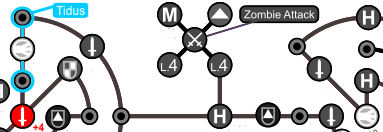
\includegraphics[width=.8\columnwidth]{graphics/tidus_bikanel}
\end{spheregrid}
\begin{enumerate}[resume]
	\item Make sure that \rikku's \od\ is full
	\item Continue along path. On the next screen, go in north-west towards the save sphere, take the shortcut to the left. Go up to the next screen and fight the Sandragora fights. They're located in the Top Right Sinkhole with Chest, and then at the end of the path up and to the left, then go up and \sd
	\item \textit{If you still have 2 Bomb Cores:}
	      \begin{itemize}
		      \item Need 4 \textit{(5 on \blitzloss)} in any combination of Sleeping Powders, Smoke Bombs, Silence Grenades
	      \end{itemize}
	\item \textit{Else:}
	      \begin{itemize}
		      \item Need 6 \textit{(7 on \blitzloss)} in any combination of Sleeping Powders, Smoke Bombs, Silence Grenades
		      \item 2 Sleeping Powders is Mandatory for the Bevelle Guards
	      \end{itemize}
\end{enumerate}
\begin{encounters}
	\begin{itemize}
		\item Prioritize Sleeping Powders over Smoke Bombs
		\item Sand Wolf steals Sleeping Powders x2
		\item Zu steals Smoke Bomb x3
		\item Alcyone steals Smoke Bomb
		      \begin{itemize}
			      \item If short on Speed Spheres, use the Smoke Bombs on them.
		      \end{itemize}
		\item \textit{Pre-Empt:}
		      \begin{itemize}
			      \tidusf Defend
			      \rikkuf Steal
			      \auronf Defend
			      \item Flee
		      \end{itemize}
		\item \textit{Neutral:}
		      \begin{itemize}
			      \switch{\tidus}{\kimahri}
			      \kimahrif Steal
			      \switch{\rikku}{\tidus}
			      \item Flee
		      \end{itemize}
		\item \textit{Else:} Flee
	\end{itemize}
\end{encounters}
\begin{battle}{Sandragora 1}
	\begin{itemize}
		\switch{\tidus}{\kimahri} or \tidus: Haste \kimahri
		\kimahrif \od\ Stone Breath
	\end{itemize}
\end{battle}
\begin{enumerate}[resume]
	\item At the bottom of the pit, \pickup{Teleport Spheres}
	\item \formation{\tidus}{\lulu}{\auron} \textit{If \blitzwin Else} \formation{\tidus}{\rikku}{\auron}
\end{enumerate}
\begin{battle}{Sandragora 2}
	\begin{itemize}
		\tidusf Haste \auron
		\auronf \od\ Shooting Star (Triangle, O, Square, X, $\leftarrow, \rightarrow$, X)
	\end{itemize}
\end{battle}
	\chapter{Home}

\begin{enumerate}
	\item Go into door, \sd
\end{enumerate}
\begin{battle}{Bombs}
	\begin{itemize}
		\tidusf Haste \tidus
		\tidusf Attach each, starting with Guado
		\auronf Attack Guado if it didn't die to \tidus
		\item \textit{\blitzloss:}
		      \begin{itemize}
			      \rikkuf Grenade
		      \end{itemize}
	\end{itemize}
	Guaranteed 6 Power Spheres.
\end{battle}
\begin{enumerate}[resume]
	\item \sd
\end{enumerate}
\begin{battle}{Dual Horn}
	\begin{itemize}
		\switch{anyone}{\kimahri}
		\kimahrif Lancet Dual Horn (Fire Breath)
		\kimahrif \od\ Stone Breath
	\end{itemize}
\end{battle}
\begin{enumerate}[resume]
	\item Heal \tidus\ without Elixirs
	\item \textit{If you \lostblitz:}
	      \begin{itemize}
		      \item Go down the stairs. Once the camera flips, \formation{\tidus}{\rikku}{\auron}, go back up the stairs into the door.
		      \item Do the following Dual Horn encounter
		            \begin{battle}{Dual Horns - \blitzloss}
			            \begin{itemize}
				            \tidusf Haste \tidus\ \textit{If no Petrify Grenade else } Defend
				            \tidusf Attack Dual Horns
				            \rikkuf 1 Petrify Grenade/Smoke Bomb/Silence Grenade (Try to keep Sleeping Powders)
				            \tidusf Attack
			            \end{itemize}
		            \end{battle}
		      	\item Open the rear chest for a \textbf{Friend Sphere}, with the codes: Bottom Middle (up x2), Middle Right (up x4), Middle (down x4) %wtf does this line mean
	      \end{itemize}
	\item \formation{\tidus}{\lulu}{\auron}
	\item Go down and left, \cs[0:50]
\end{enumerate}
\begin{battle}{Chimera}
	\begin{itemize}
		\switch{anyone}{\kimahri}
		\kimahrif Lancet Chimera (Aqua Breath)
		\kimahrif \od\ Stone Breath
	\end{itemize}
\end{battle}
\begin{enumerate}[resume]
	\item Walk down steps, \cs[1:30]
	\item Before going further, \pickup{Level 2 Key Sphere}
	\item \sd\ until Tidus asks ``why'', \cs[6:20]
	\item \formation{\tidus}{\rikku}{\kimahri}
	\item Go bottom right to the next screen, run across the bridge
\end{enumerate}
\newpage
	\chapter{Airship}

\begin{enumerate}
	\item \sd\ during \cs+3 \skippablefmv. Walk down corridor to the next screen, go back in, \sd. Speak to Brother, \sd. Walk towards corridor, \sd. Walk towards camera to the next screen, go up and speak to Rin.
	\item If missing any spheres, buy Distillers from Rin either the first time you see him or right before Evrae Altana. Each one counts as 2 Spheres.
	\item \save. Make sure that \rikku\ has \od. If she doesn't, you can get encounters on Rin's first screen.
\end{enumerate}
\begin{battle}[32000]{Evrae}
	\begin{itemize}
		\item \textit{If you \wonblitz:}
		      \begin{itemize}
			      \tidusf Haste \tidus
			      \tidusf Cheer
			      \tidusf If \tidus\ is still going next, Change Armor
			      \rikkuf \od\ Mix Luck Sphere + Map
			      \tidusf Attack x2
			      \tidusf Cheer
			      \tidusf Attack x3
			      \kimahrif Heal \tidus\ if he was hit in the first attack, Steal otherwise
			      \rikkuf Steal
		      \end{itemize}
		\item \textit{If you \lostblitz:}
		      \begin{itemize}
			      \tidusf Haste \tidus
			      \tidusf Cheer x2
			      \tidusf Equip Baroque Sword
			      \tidusf Attack x6
			      \rikkuf \od\ Mix Luck Sphere + Map
			      \item \kimahri\ or \rikku: Full Heal \tidus, Lunar Curtain \tidus
			      \item \kimahri\ or \rikku: Steal
		      \end{itemize}
	\end{itemize}
\end{battle}
\begin{enumerate}[resume]
	\item \sd, \skippablefmv[3:00] - Press Start immediately after the FMV.
\end{enumerate}
\vfill
\ 
\columnbreak
\newline
	\chapter{Bevelle}
\begin{enumerate}
	\item Use a Mega-Potion
	\ifthenelse{\equal{\blitzresult}{win}}{}{
		\ifthenelse{\equal{\blitzresult}{both}}{
			\item \textit{If you \lostblitz:}
	}{}
		\begin{equip}
			\begin{itemize}
				\tidusf Equip Sonic Steel
			\end{itemize}	
		\end{equip}
	}
	\item \textit{With Sleeping Powder:}
\end{enumerate}
\begin{battle}{Guard Fights - Sleeping Powder}
	\begin{itemize}
		\item \textit{Fights 1 and 3 (3 Monks):}
			\begin{itemize}
				\tidusf Attack
				\item Others: Defend or use Distillers
			\end{itemize}
		\item \textit{Fights 2 and 4 (2 Monks and a YKT-63):}
			\begin{itemize}
				\tidusf Attack the YKT-63
				\rikkuf Sleeping Powder
				\kimahrif Smoke Bomb/Silence Grenade/Sleeping Powder/Distiller
			\end{itemize}
		\item \textit{Fight 5 (2 Monks and a YAT-99):}
			\begin{itemize}
				\item \textit{If you have 2 Smoke Bombs/Sleeping Powders/Silence Grenades:}
					\begin{itemize}
						\tidusf Haste \rikku
						\rikkuf Sleeping Powder/Smoke Bomb/Silence Grenade
						\rikkuf If the Guards are sleeping use a Bomb Core on the YAT-99
						\rikkuf Sleeping Powder/Smoke Bomb/Silence Grenade
						\tidusf Attack
					\end{itemize}
				\item \textit{If you have 2 Bomb Cores:}
					\begin{itemize}
						\tidusf Attack the Monks
						\item Others: Use Bomb Core x2 on the YAT-99
					\end{itemize}
			\end{itemize}
	\end{itemize}
\end{battle}
\bothvfill
\lossvfill
\winvfill
\ 
\bothcb
\wincb
\losscb
\ 
\ \bothnewline \winnewline \lossnewline
\begin{enumerate}[resume]
	\item \textit{Without Sleeping Powder:}
		\begin{itemize}
			\item Keep \formation{\tidus}{\rikku}{\lulu} for the first 4 fights, \formation{\tidus}{\rikku}{\kimahri} for the last one
		\end{itemize}
\end{enumerate}
\begin{battle}{Guard Fights - No Sleeping Powder}
	\begin{itemize}
		\item \textit{Fights 1 and 3 (3 Monks):}
			\begin{itemize}
				\tidusf Attack
				\item Others: Defend or use Distillers
			\end{itemize}
		\item \textit{Fights 2 and 4 (2 Monks and a YKT-63):}
			\begin{itemize}
				\switch{\tidus}{\kimahri}
				\kimahrif Silence Grenade/Smoke Bomb
				\rikkuf Silence Grenade/Smoke Bomb
				\switch{\kimahri}{\tidus}
				\tidusf Attack the YKT-63
				\item \textit{If the YKT-63 is still alive} Use a Lightning Marble/Arctic Wind/Fish Scale or Attack with \tidus
			\end{itemize}
			\item \textit{Fight 5 (2 Monks and a YAT-99):}
			\begin{itemize}
				\item \textit{If you have 2 Smoke Bombs/Silence Grenades:}
					\begin{itemize}
						\tidusf Haste \rikku
						\rikkuf Smoke Bomb/Silence Grenade x2
						\tidusf Attack
					\end{itemize}
				\item \textit{If you have 2 Bomb Cores:}
					\begin{itemize}
						\tidusf Attack the Monks
						\item Others: Use Bomb Core x2 on the YAT-99
					\end{itemize}
			\end{itemize}
	\end{itemize}
\end{battle}
\begin{enumerate}[resume]
	\item \sd, \skippablefmv[1:30], \sd\ on \yuna\ dialogue. \skippablefmv[30], \sd. Use lift, \sd.
\end{enumerate}
\bothvfill
\winvfill
\lossvfill
\ 
\begin{trial}
	\begin{itemize}
		\item \textit{Upper section:}
			\begin{itemize}
				\item Push the pedestal in
				\item Press X
				\item Go left at the 2nd junction
				\item Take sphere, push pedestal back
				\item At the 3rd junction, go back (hold X)
				\item Go left at the 2nd junction
				\item Place sphere into wall, push pedestal back
				\item At the 3rd junction, go back (hold X)
				\item Go left at the 1st junction
			\end{itemize}
		\item \textit{Lower section (1st visit):}
			\begin{itemize}
				\item The platform will automatically stop at the 1st junction
				\item After the platform stops, press X the 2nd time the arrow is pointing left
				\item Go right at the 3rd junction (hold X after the 2nd junction)
				\item Take Glyph sphere from wall, push pedestal back
				\item At the 4th junction go right (hold X)
				\item Place Glyph sphere into pedestal
				\item Take Bevelle sphere from pedestal
				\item Place Bevelle sphere into the wall
				\item Take the Glyph sphere
				\item Place Glyph sphere into the next wall
				\item Take Destruction sphere from the new wall
				\item Place Destruction sphere on the pedestal
				\item Take Bevelle sphere from the wall
				\item Push pedestal back and fall off the edge
			\end{itemize}
		\item \textit{Lower section (2nd visit):}
			\begin{itemize}
				\item Go straight (hold X)
				\item At the 3rd junction go right (hold X after the 2nd junction)
				\item Place Bevelle sphere on the pedestal
				\item Take Destruction sphere from the pedestal
				\item Place Destruction sphere into wall
				\item Push pedestal back and fall off the edge
			\end{itemize}
		\item \textit{Lower section (3nd visit):}
			\begin{itemize}
				\item Go straight
				\item At the 2nd junction go right (hold X)
				\item Push pedestal
				\item Go up the stairs, open the chest
			\end{itemize}
	\end{itemize}
\end{trial}
\begin{enumerate}[resume]
	\item \sd, name \bahamut, don't save, \sd
\end{enumerate}
\lossvfill
\ 
\losscb
\ \lossnewline \ 

	\chapter{Via Purifico}

\begin{enumerate}
	\item Run up past the first telepad
	\item Go to the second telepad and travel north.
\end{enumerate}
\begin{spheregrid}
	\begin{itemize}
		\auronf
		\begin{itemize}
			\item Move $\rightarrow\rightarrow\rightarrow$
			\item Level 2 Keysphere
			\item Move $\rightarrow\rightarrow\rightarrow\rightarrow$
			\item Level 2 Keysphere
			\item Move $\uparrow\uparrow$
			\item Mag+3
		\end{itemize}
		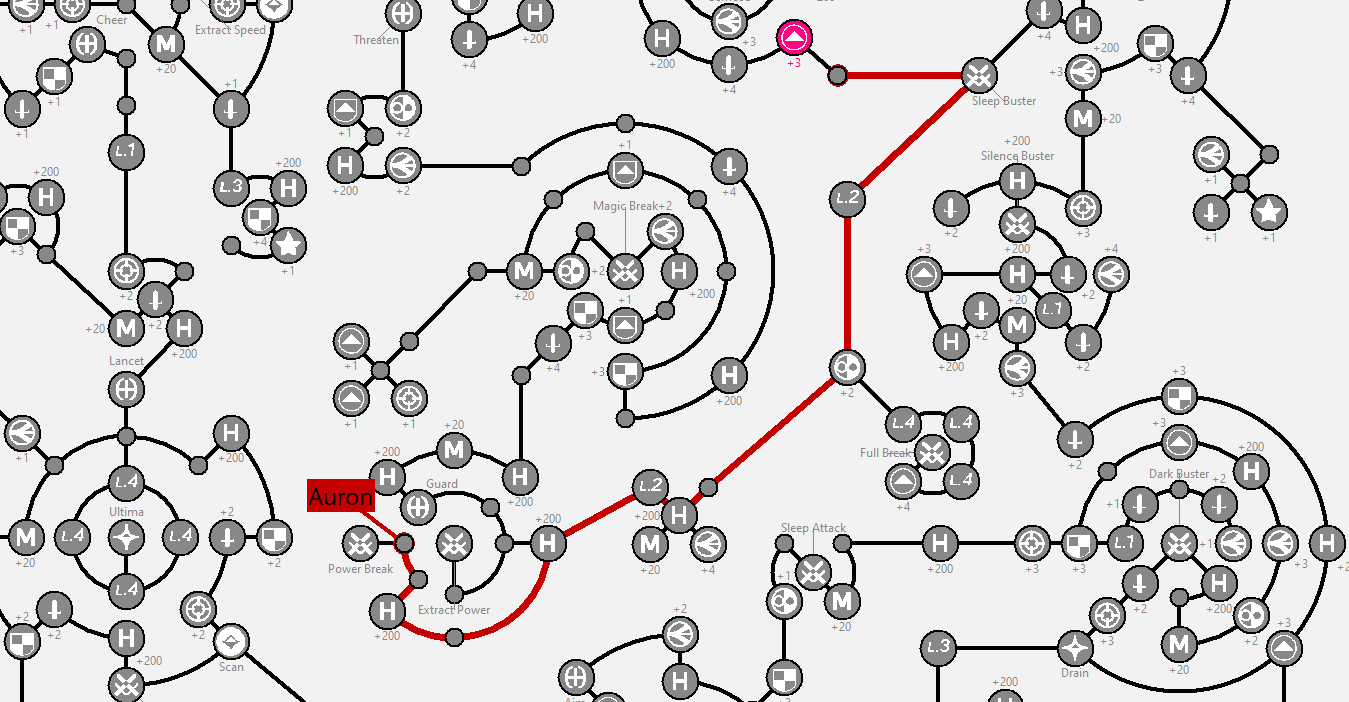
\includegraphics[width=.8\columnwidth]{graphics/Auron_Via_Purifico}
		\yunaf
		\begin{itemize}
			\item Teleport Sphere to Auron's Magic Node $\uparrow$
			\item Mag+3, Str+4
			\item Move $\rightarrow\rightarrow\rightarrow\uparrow$
			\item HP+200, Str+4, Mag+3
			\item Move $\rightarrow$
			\item Def+3, Str+4, Agi+3
			\item Move $\swarrow\downarrow$
			\item MP+20
			\item Move $\swarrow$
			\item HP+200, Str+2
			\item Move $\downarrow$
			\item Str+2
		\end{itemize}
		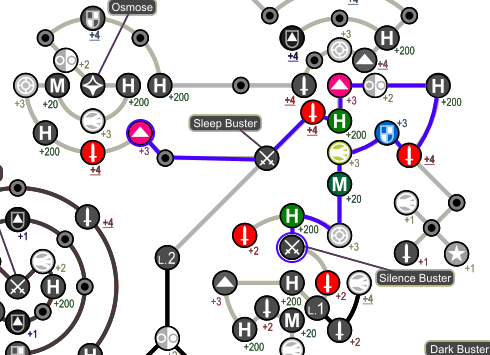
\includegraphics[width=.8\columnwidth]{graphics/Yuna_Via_Purifico}
	\end{itemize}
\end{spheregrid}
\begin{enumerate}[resume]
	\item Check how many Power Spheres you have left, you need 15 more for the rest of the run
	\item Keep track of how many things you kill here.
\end{enumerate}
\begin{encounters}
	\begin{itemize}
		\item Maze Larva: Summon \ixilon, Attack
	\end{itemize}
\end{encounters}
\bothvfill
\lossvfill
\begin{battle}{Isaaru}
	\begin{itemize}
		\item Grothia (8000 HP):
		      \begin{itemize}
			      \summon{\bahamut}
			      \bahamutf Attack
		      \end{itemize}
		\item Pterya (12000 HP):
		      \begin{itemize}
			      \summon{\bahamut}
			      \bahamutf Attack x2
		      \end{itemize}
		\item Spathi (12000 HP):
		      \begin{itemize}
			      \summon{\ixilon}
			      \ixilonf Attack x5
		      \end{itemize}
	\end{itemize}
\end{battle}
\begin{enumerate}[resume]
	\item Swim right and then up. Can use the underwater chest at the start to buy Power Distillers. If needed, you can attack Yellow Starfish and Sahagins with \tidus\ for 2x Power Spheres.
\end{enumerate}
\begin{battle}{Evrae Altana}
	\begin{itemize}
		\item Anyone: 1 Power Distiller if needed
		\item Anyone: Phoenix Down x2/Elixir Evrae Altana
	\end{itemize}
\end{battle}
\begin{enumerate}[resume]
	\item Swim to exit, \sd
\end{enumerate}
\bothvfill
\bothnp
	\chapter{Highbridge}
\begin{spheregrid}
	\begin{itemize}
		\yunaf
		\blitzballSphereGrid{%
		      \item Teleport to Strength Sphere $\uparrow\uparrow$ or $\nearrow$
		      \item Str+4, Str+4, Def+3
		      \item Move $\leftarrow\leftarrow$
		      \item Str+4, HP+200, Agi+2
		      \item Move $\leftarrow$
		      \item Str+4
		      \item Move $\leftarrow\leftarrow\leftarrow\leftarrow$
		      \item Str+4
		}{.9}{graphics/Yuna_blitz_WIN_highroad}{%
		      \item Teleport to \tidus\ Str+4 by Mental Break $\leftarrow$
		      \item Str+4, HP+200
		      \item Friend Sphere to \tidus\ $\uparrow$
		      \item Agi+2, Str+4
		      \item Move $\rightarrow\rightarrow$
		      \item Str+4
		      \item Move $\rightarrow\rightarrow\rightarrow\rightarrow$
		      \item Str+4
		      \item Move $\uparrow$
		      \item Str+4\newline
		}{.9}{graphics/Yuna_blitz_loss_highbridge_1}
	\end{itemize}
\end{spheregrid}
\begin{enumerate}
	\item Walk north
	\item From this point on, watch any pre-empts if \yuna\ is in the party, because she can get the first turn. Check to make sure that \lulu\ has 35 levels.
	\item \formation{\tidus}{\yuna}{\auron}
	\item Need 4 Maze Larva/YKT-63 Kills total, Overkills count as 1.
\end{enumerate}
\bothvfill
\winvfill
\begin{encounters}
	\begin{itemize}
		\item YKT-63:
		      \begin{itemize}
			      \tidusf Attack
			      \yunaf Attack
			      \item Flee
		      \end{itemize}
	\end{itemize}
\end{encounters}
\bothvfill
\begin{battle}[36000]{Seymour Natus}
	\begin{itemize}
		\item \textit{If \lulu\ has less than 35 levels:}
		      \begin{itemize}
			      \switch{\tidus}{\lulu}
			      \luluf Switch Weapon
			      \switch{\lulu}{\tidus}
		      \end{itemize}
		      \tidusf Attack
		      \summon{\bahamut}
		      \bahamutf Attack
	\end{itemize}
\end{battle}
\begin{enumerate}[resume]
	\item \sd
	\item Walk to \yuna, \cs+\skippablefmv[10:10]. Walk down, \cs[1:40], walk right, exit Macalania Woods
\end{enumerate}
	\chapter{Calm Lands}

\begin{enumerate}
	\item \sd, walk left
\end{enumerate}
\begin{spheregrid}
	\begin{itemize}
		\yunaf
		\blitzballSphereGrid{%
			      \item Move $\leftarrow$
			      \item Str+4
			}{.5}{graphics/yuna_blitz_win_highbridge_2}{%
			      \item Move $\rightarrow$
			      \item Str+4, Def+3
			}{.5}{graphics/yuna_blitz_loss_highbridge_2}
	\end{itemize}
\end{spheregrid}
\begin{enumerate}[resume]
	\item \textit{If you only have 1 \textbf{Water Gem}:} \formation{\tidus}{\auron}{\yuna}, then make sure to do a Flame Flan Encounter
\end{enumerate}
\begin{encounters}
	\begin{itemize}
		\item Flame Flan:
		      \begin{itemize}
			      \switch{anyone}{\kimahri}
			      \kimahrif Steal
			      \switch{anyone}{\tidus}
			      \item Flee
		      \end{itemize}
	\end{itemize}
\end{encounters}
\begin{enumerate}[resume]
	\item \formation{\tidus}{\kimahri}{\auron}
	\item Continue north to the Calm Lands Exit
	\item Run north, \sd
\end{enumerate}
\begin{battle}[64000]{Defender X}
	\begin{itemize}
		\switch{\tidus}{\yuna}
		\summon{\bahamut}
		\bahamutf Attack x2
	\end{itemize}
\end{battle}
\begin{enumerate}[resume]
	\item \sd, walk across bridge and up to Mt. Gagazet, \sd
\end{enumerate}
\bothvfill
\lossvfill
\ 
\bothcb
\losscb
\newline

	\chapter{Mt. Gagazet}
\begin{enumerate}
	\item Walk up, \cs[3:40], walk up, \sd
\end{enumerate}
\begin{battle}{Biran and Yenke}
	\begin{itemize}
		\kimahrif Steal from Biran
		\kimahrif Gem Yenke
		\kimahrif Gem Biran
	\end{itemize}
	Pay attention to your drops, they affect \yuna's sphere grid below.
\end{battle}
\end{multicols}
\begin{spheregrid}
	\begin{multicols}{2}
		\begin{itemize}
			\luluf
			\begin{itemize}
				\item Move $\uparrow\uparrow$
				\item Level 2 Key Sphere
				\item Move $\downarrow x9$
				\item Level 3 Key Sphere
				\item Move $\searrow\searrow$
			\end{itemize}
			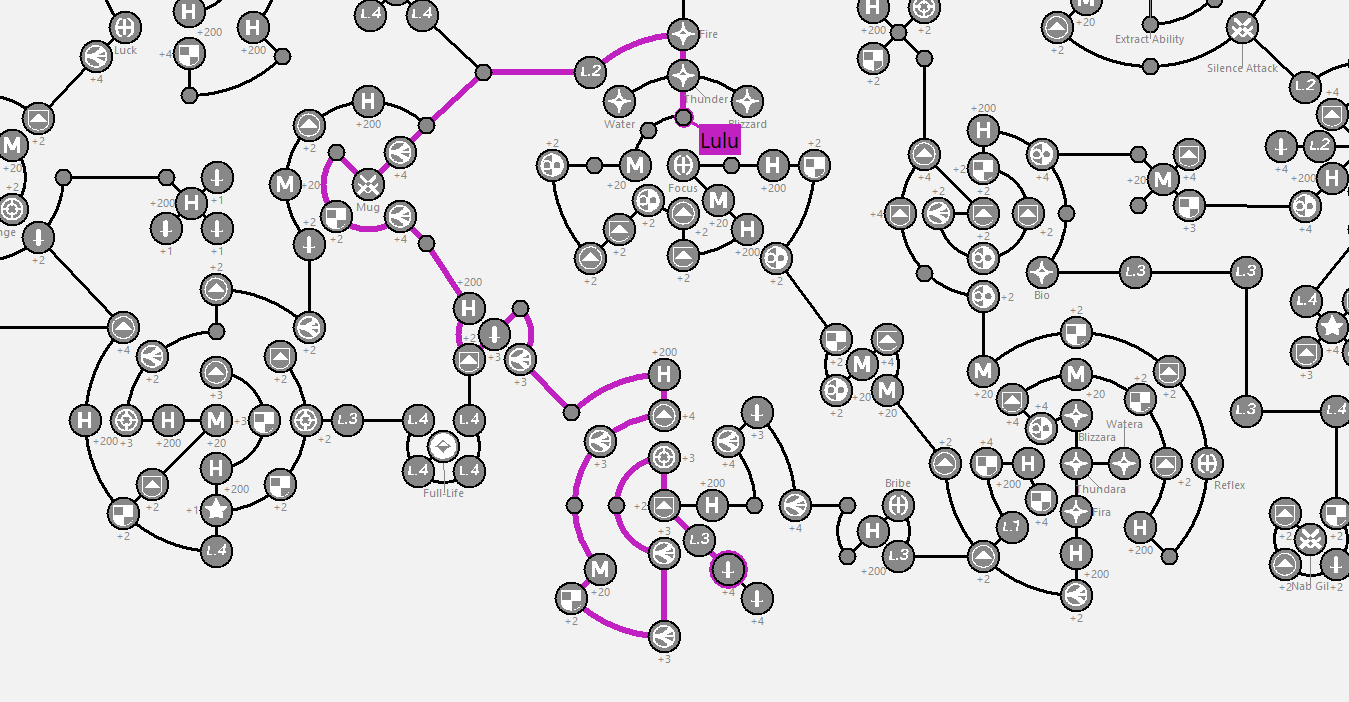
\includegraphics[width=.75\columnwidth]{graphics/lulu_grid}
			\yunaf
			\begin{itemize}
				\item \textit{If you got \textbf{4 Return Spheres}:}
				      \begin{itemize}
					      \item Return to the last Str+2 node in \wakka's grid, Hold $\searrow$
					      \item Move $\leftarrow$
					      \item Mag+3, Level 1 Key Sphere
					      \item Move $\downarrow\downarrow$
					      \item Str+2, Agi+4
				      \end{itemize}
				      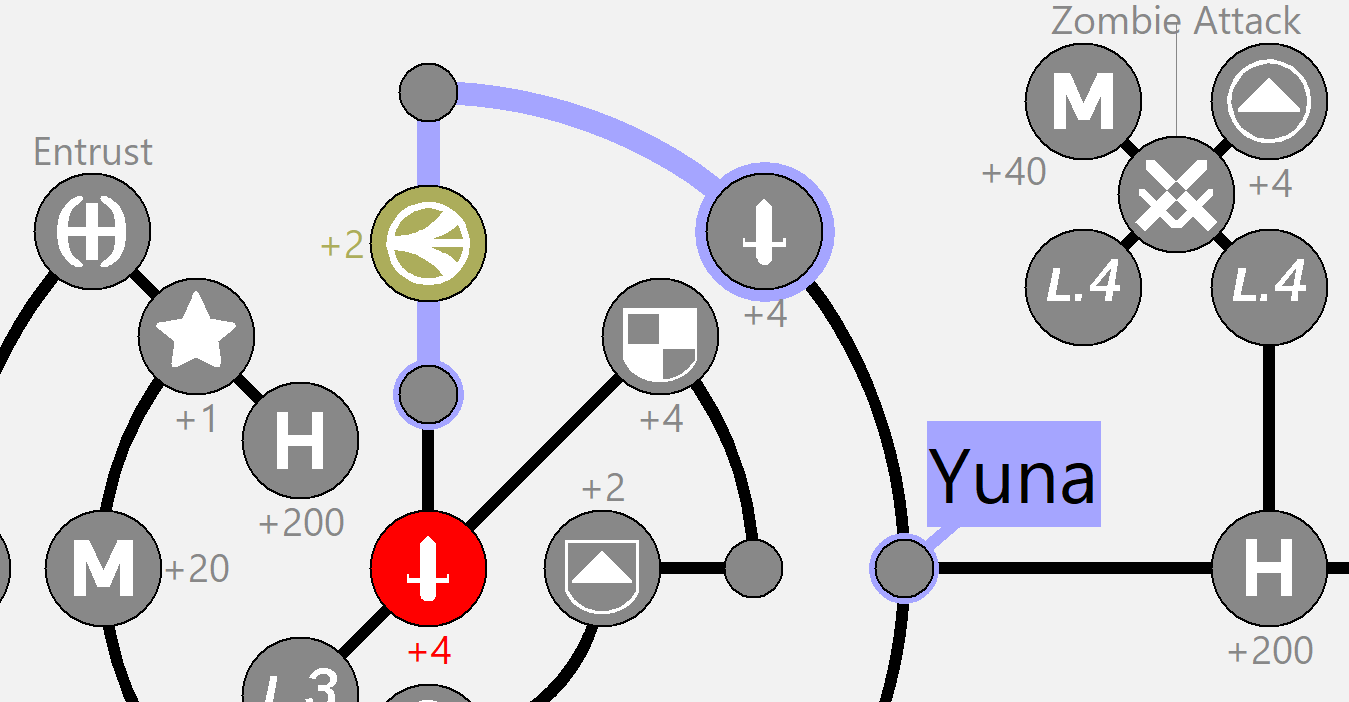
\includegraphics[width=.5\columnwidth]{graphics/4_returns_1}
				\item \textit{If you got \textbf{2 Return Spheres}:}
				      \begin{itemize}
					      \item Friend Sphere to \lulu,  $\downarrow\downarrow$
					      \item Str+4, Str+4
					            \luluf Move $\nearrow\uparrow\uparrow$
					            \yunaf Friend Sphere to \lulu,
					      \item Str+3, Agi+4, Agi+4
				      \end{itemize}
				      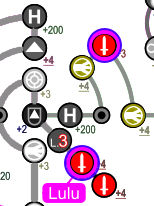
\includegraphics[width=.4\columnwidth]{graphics/2_and_2}
				      \columnbreak
				\item \textit{If you got \textbf{0 Return Spheres}:}
				      \begin{itemize}
					      \tidusf Move to Str+4 by Mental Break $\rightarrow x3, \downarrow, \rightarrow x3$
					      \yunaf Friend Sphere to \tidus
					      \item Str+4
					            \tidusf Move $\nwarrow\leftarrow$ or $\swarrow\swarrow$
					      \item Armor Break
					      \item Do the 2 Return Sphere Menu
					            \rikkuf: Move $\downarrow x5$
					            \yunaf Friend to \rikku\ $\downarrow$
					      \item Agi+4, MgDef +2
					      \item Move $\leftarrow$
					      \item Str+2
				      \end{itemize}
				      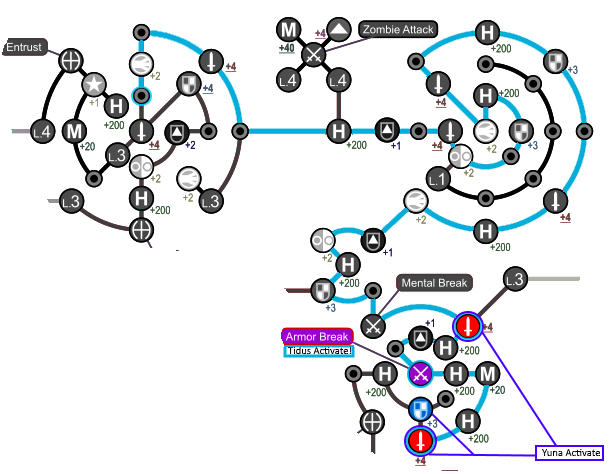
\includegraphics[width=.9\columnwidth]{graphics/0_returns}
				      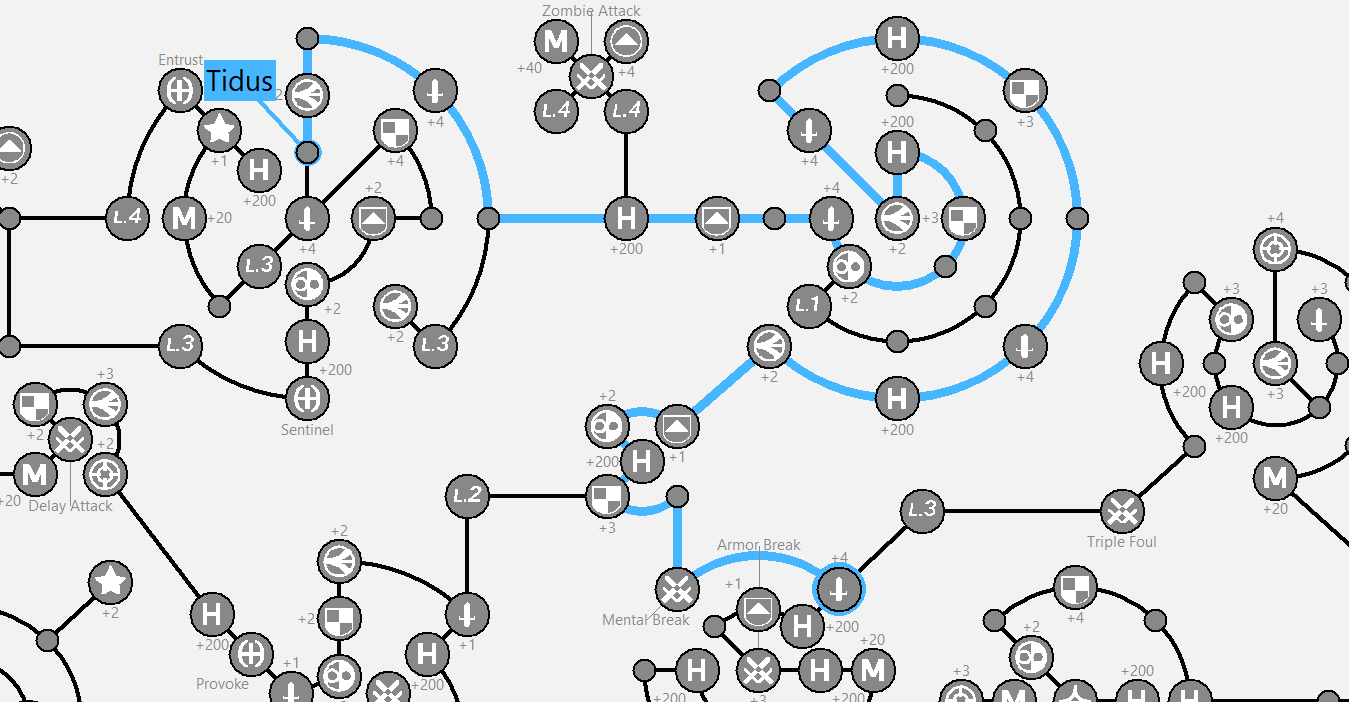
\includegraphics[width=.7\columnwidth]{graphics/0_returns_pt2}
			\end{itemize}
			\item \tidus\ \textit{if you didn't get Armor Break:}
			      \begin{itemize}
				      \item \textit{If you got \textbf{4 Return Spheres}:}
				            \begin{itemize}
					            \item Return Sphere $\downarrow\searrow\searrow$, Str+4 near Armor Break
					            \item Move $\nwarrow\leftarrow$ or $\swarrow\swarrow$
				            \end{itemize}
				      \item \textit{If you got \textbf{2 Return Spheres}:}
				            \begin{itemize}
					            \item Move to Armor Break $\rightarrow x3, \downarrow x6$
				            \end{itemize}
				      \item Armor Break
			      \end{itemize}

		\end{itemize}
	\end{multicols}
\end{spheregrid}
\begin{multicols}{2}
\begin{enumerate}[resume]
	\item \textit{If you had 2 or 4 \textbf{Return Spheres}:}
	      \begin{itemize}
		      \item Customize:
		            \begin{itemize}
			            \auronf Shimmering Blade $\rightarrow$ First Strike
			            \yunaf Staff $\rightarrow$ First Strike
		            \end{itemize}
	      \end{itemize}
	\item \formation{\tidus}{\rikku}{\auron} \textit{If you need need to build up \rikku\ \od\ else } \formation{\tidus}{\kimahri}{\wakka}.
\end{enumerate}

\begin{equip}
	\begin{itemize}
		\auronf Sonic Blade
	\end{itemize}
\end{equip}
\begin{enumerate}[resume]
	\item Walk up, \sd, \cs[1:20], continue walking up, avoid the gravestones.
	\item Make sure you charge \rikku's \od, can skip if you still have a Silence Grenade
	\item Follow the path around.
	\item Once you're on the Seymour Flux screen, if you're using \rikku\ \od, then Hi-Potion Rikku
	\item \formation{\tidus}{\yuna}{\auron} \textit{If you had 2 or 4 Return Spheres else } \formation{\tidus}{\kimahri}{\wakka}
\end{enumerate}
\begin{battle}[70000]{Seymour Flux}
	\begin{itemize}
		\item \textit{If you had 2 or 4 \textbf{Return Spheres}:}
		      \begin{itemize}
			      \yunaf Attack
			      \tidusf Haste \yuna
			      \switch{\auron}{\rikku}
			      \rikkuf Silence Grenade or \od\ HP Sphere + Grenade
			      \summon{\bahamut}
			      \bahamutf Impulse
			      \yunaf Attack
			      \tidusf Attack. If \yuna\ crit, skip the second Attack to try and get Overkill
		      \end{itemize}
		\item \textit{If you had 0 \textbf{Return Spheres}:}
		      \begin{itemize}
			      \switch{\tidus}{\yuna}
			      \summon{\bahamut}
			      \bahamutf Attack
		      \end{itemize}
	\end{itemize}
\end{battle}
\begin{enumerate}[resume]
	\item \formation{\tidus}{\kimahri}{\auron}
	\item \save\ if \bahamut was banished, Walk to the next screen. \skippablefmv[0:20], \sd, walk up to \tidus\ House, go into the center, \sd. Follow the boy outside, speak to him upstairs, \sd.
	\item Walk up to the next screen, go up the steps. Go down the left path into the water, \sd, swim up. Go up the steps, play the minigame, return to the previous screen.
	\item \tidus\ can attack Splashers for Power Spheres if needed. Try to only attack the 3 fish groups.
	\item Return to Save Sphere, go up and left, then go down the right path, swim up into the next screen. Complete the minigame, \rikku\ Green, \tidus\ Blue, \wakka\ Red. Return.
	\item Go up left path, \sd, continue up the path, \save\ if \bahamut\ was banished and you didn't touch one earlier.
	\item \formation{\tidus}{\yuna}{\kimahri}. Go onto the next screen.
\end{enumerate}
\begin{battle}[40000]{Sanctuary Keeper}
	\begin{itemize}
		\item \textit{If 2 or 4 \textbf{Return Spheres}:}
		      \begin{itemize}
			      \yunaf Defend
			      \tidusf Armor Break
		      \end{itemize}
		\item \textit{If 0 \textbf{Returns Spheres}:}
		      \begin{itemize}
			      \tidusf Defend
		      \end{itemize}
		      \summon{\bahamut}
		      \bahamutf Attack
	\end{itemize}
\end{battle}
	\chapter{Zanarkand}
\begin{enumerate}
	\item \sd, \cs[0:50], walk left. \fmv+\cs[2:20]
	\item Move left to the sphere, \sd, \cs[1:40]. Walk further left and follow the path down, \cs[3:20], walk left onto the next screen.
	\item \formation{\tidus}{\auron}{\kimahri} \textit{if you don't need to build \rikku\ \od\ else} \formation{\tidus}{\auron}{\rikku}.
	\item Make sure to build \rikku\ \od\ on Behemoth or Defender Z, unless you want to use a Skill Sphere on the Final Boss for Armor Break.
	\item If you missed the Overkill on \textbf{Seymour Flux}, then kill two \textbf{YKT-11} or one \textbf{Defender Z} with \yuna\ and \tidus, with \formation{\tidus}{\yuna}{\auron}. Only \yuna\ needs the AP.
\end{enumerate}
\begin{encounters}
	\begin{itemize}
		\item YKT-11:
		      \begin{itemize}
			      \tidusf Attack
			      \yunaf Attack
		      \end{itemize}
		\item Singular Defender Z Inside of Dome:
		      \begin{itemize}
			      \summon{\bahamut}
			      \bahamutf Attack
		      \end{itemize}
	\end{itemize}
\end{encounters}
\begin{enumerate}[resume]
	\item Continue on the path. \pickup{Fortune Sphere} on the left of the road. Seymour's Mom \cs
	\item After the \cs, \pickup{Friend Sphere} on the right, \textbf{skip} it if you had 0 or 2 Return Spheres. When you leave the last encounter zone, the hallway before the Zanarkand Trials, \pickup{Luck Sphere} on the right.
\end{enumerate}
\bothvfill
\bothnp
\winvfill
\winnp
\lossvfill
\lossnp
\begin{spheregrid}
	\begin{itemize}
		\yunaf
		\begin{itemize}
			\item \textit{If you got \textbf{4 Return Spheres}:}
			      \begin{itemize}
				      \item Friend Sphere to \lulu\ $\downarrow\downarrow$
				      \item Luck Sphere, Fortune Sphere
				      \item Str+4, Str+4
				      \item Move $\nearrow\uparrow\uparrow$
				      \item Agi+4, Agi+4, Str+3
			      \end{itemize}
			      \ifthenelse{\equal{\colstyle}{multi}}{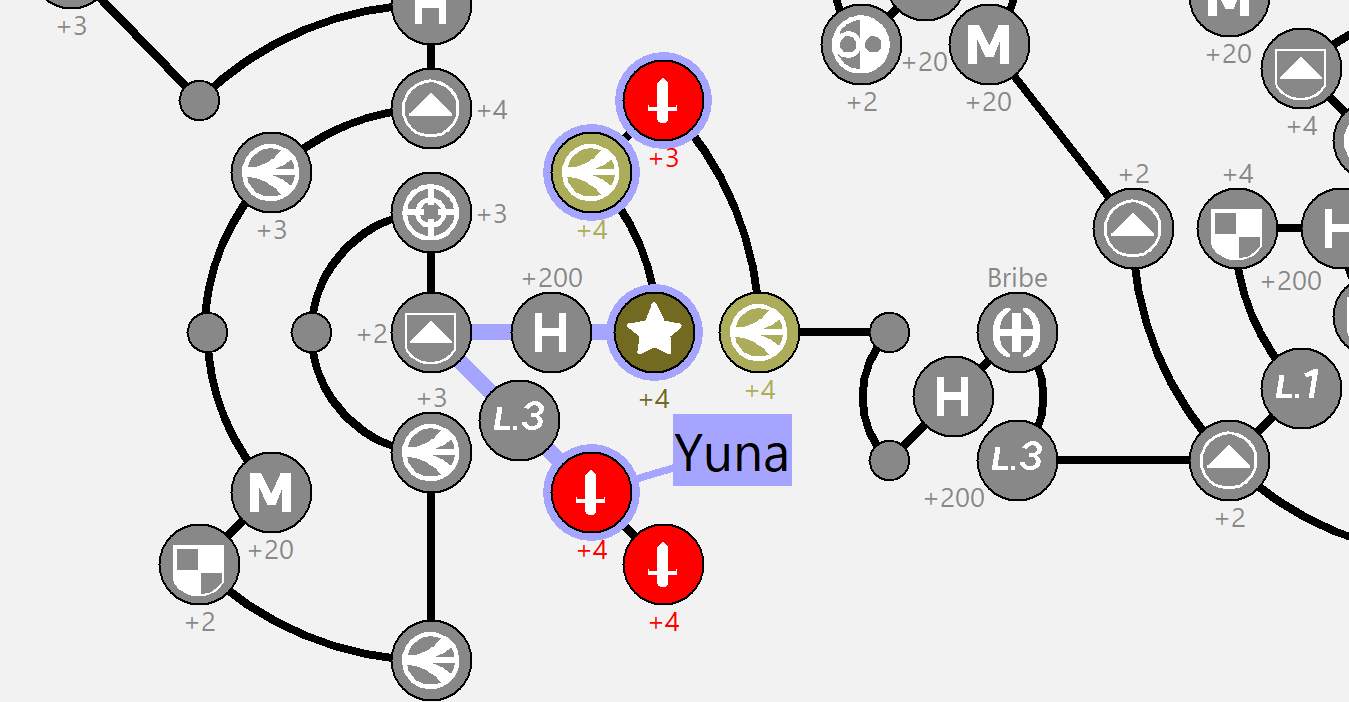
\includegraphics[width=.5\columnwidth]{graphics/4_returns_w_luck_pt1}}{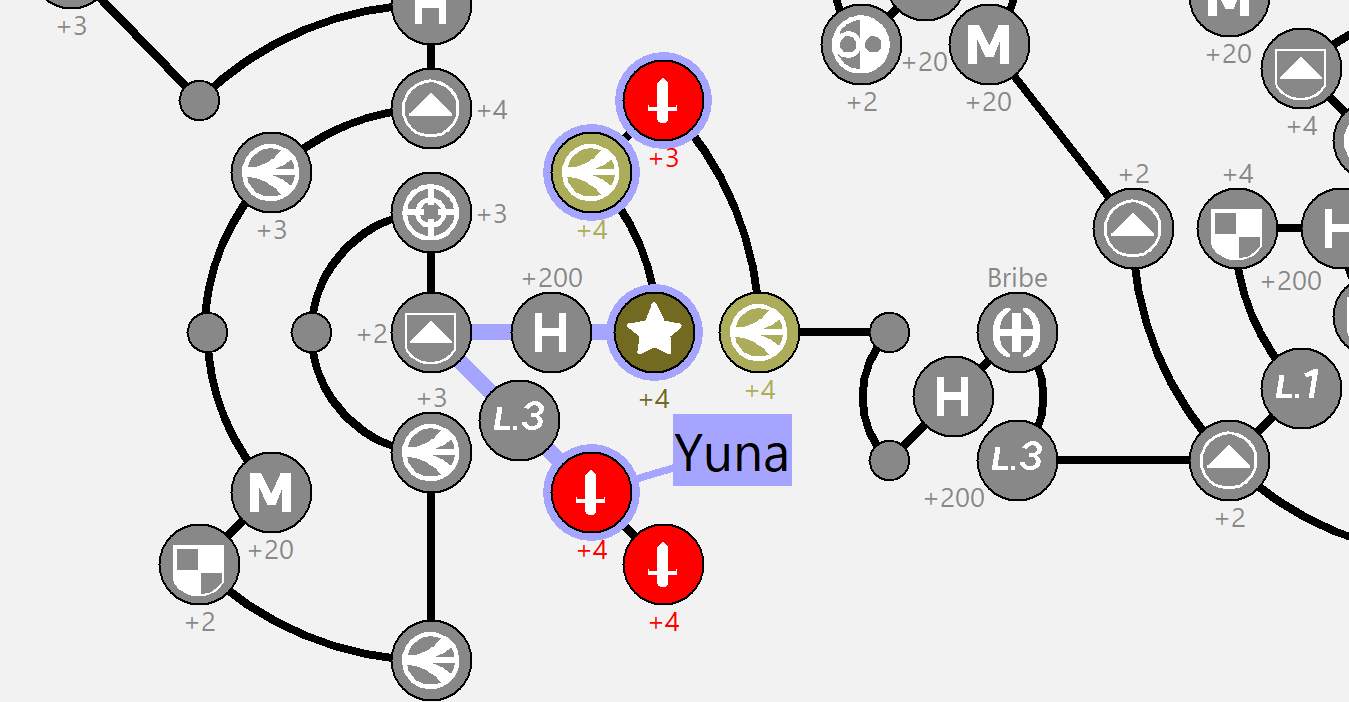
\includegraphics[width=.2\columnwidth]{graphics/4_returns_w_luck_pt1}}
			\item \textit{If you got \textbf{2 Return Spheres}:}
			      \begin{itemize}
				      \item Return Sphere to Str+2 in \wakka's grid, $\nearrow$
				      \item Move $\leftarrow$
				      \item Level 1 Key Sphere, Mag+3
				      \item Luck Sphere, Fortune Sphere
				      \item Move $\searrow\searrow$
				      \item Agi+4, Str+2
				      \item Move $\leftarrow\leftarrow$
				      \item Agi+3, Str+2
				      \item Move $\downarrow$
				      \item Str+2
			      \end{itemize}
			      \ifthenelse{\equal{\colstyle}{multi}}{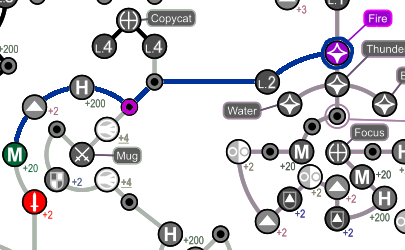
\includegraphics[width=.5\columnwidth]{graphics/2_and_2_with_luck}}{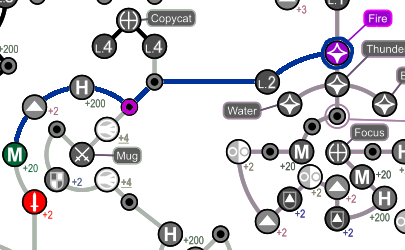
\includegraphics[width=.2\columnwidth]{graphics/2_and_2_with_luck}}
			\item \textit{If you got \textbf{0 Return Spheres}:}
			      \begin{itemize}
				      \item Move $\downarrow\downarrow$
				      \item Luck Sphere, Fortune Sphere
			      \end{itemize}
			      \ifthenelse{\equal{\colstyle}{multi}}{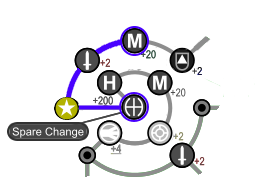
\includegraphics[width=.7\columnwidth]{graphics/0_return_w_luck}}{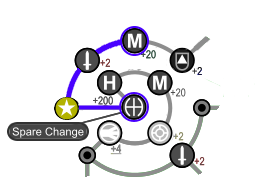
\includegraphics[width=.25\columnwidth]{graphics/0_return_w_luck}}
		\end{itemize}
	\end{itemize}
\end{spheregrid}
\bothcb \wincb \losscb
\begin{enumerate}[resume]
	\item \formation{\tidus}{\auron}{\yuna}
	\item \textit{If you had 0 Return Spheres:}
	      \begin{itemize}
		      \item Customize:
		            \begin{itemize}
			            \auronf Shimmering Blade $\rightarrow$ First Strike
			            \yunaf Staff $\rightarrow$ First Strike
		            \end{itemize}
	      \end{itemize}
\end{enumerate}
\begin{equip}
	\begin{itemize}
		\auronf Sonic Blade
	\end{itemize}
\end{equip}
\begin{enumerate}[resume]
	\item {\large \save}
\end{enumerate}
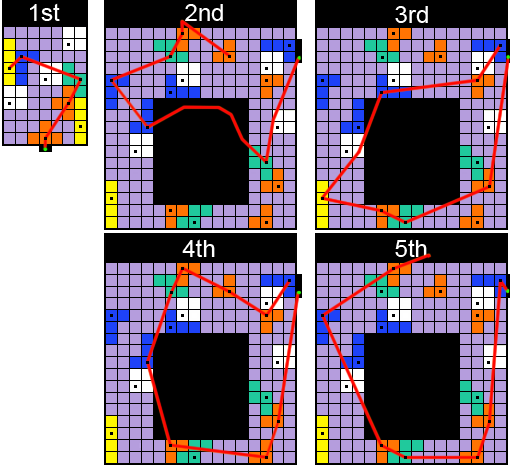
\includegraphics[width=.95\columnwidth]{graphics/Zanarkand_Trials}
\begin{enumerate}[resume]
	\item Push in the pedestals starting from the Top Left, to Bottom Left, then Top Right, Bottom Right, then Besaid Sphere. After pushing in each pedestal, do the corresponding puzzle, shown above.
	\item After the second puzzle, take the Kilika Sphere on the left and put it into the second pedestal.
	\item After the fifth puzzle, take the Besaid Sphere from the right and put it into the fifth pedestal.
	\item \cs, run into the large room
\end{enumerate}
\begin{battle}[52000]{Spectral Keeper}
	\begin{itemize}
		\summon{\bahamut}
		\bahamutf Attack
	\end{itemize}
\end{battle}
\bothvfill\winvfill\lossvfill
\begin{spheregrid}
	\begin{itemize}
		\item \textit{If you had 4 \textbf{Return Spheres}}:
		      \begin{itemize}
			      \item Return Sphere to Mag+3 in \wakka's Grid, $\uparrow\rightarrow\downarrow$ or $\nearrow$
			      \item Move $\rightarrow$
			      \item Str+2
			      \item Move $\downarrow\downarrow$
			      \item Str+2, Agi+3
		      \end{itemize}
		\item \yuna\ should have 70 Str and 35 Agi. If short, then the key Str Nodes are near \tidus's Armor Break and the end of \wakka's grid, and Agi is near \lulu\ (+8), \rikku\ (+3) and \wakka\ (+3 near Mag+3). If you need more Return Spheres to do these, then you can attack Sinspawn Genais for an extra one, though it costs 26 seconds
	\end{itemize}
	\ifthenelse{\equal{\colstyle}{multi}}{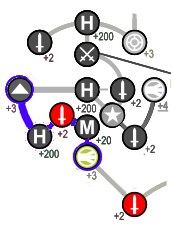
\includegraphics[width=.5\columnwidth]{graphics/4_return_before_yunalesca}}{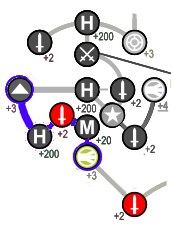
\includegraphics[width=.25\columnwidth]{graphics/4_return_before_yunalesca}}
\end{spheregrid}
\begin{enumerate}[resume]
	\item \save, Run up, \sd by mashing another button (like \textbf{R1}) at the same time as confirm, walk up to Yunalesca's room, \sd
\end{enumerate}
\begin{battle}[132000]{Yunalesca}
	\begin{itemize}
		\summon{\bahamut}
		\bahamutf Attack
	\end{itemize}
	Check for any weapon drops with \textbf{Zombie Strike}
\end{battle}
\begin{enumerate}[resume]
	\item \sd, leave room, walk down steps, \sd, go down on the next screens, \save, go up the lift, walk out of the cloister of trials, walk down the steps, walk down, \sd\ during \cs+\skippablefmv
\end{enumerate}
	\chapter{Airship}
\begin{enumerate}
  \item \sd, walk out of the cockpit past Rin, along the corridors to \yuna\ and \kimahri. \sd. Walk back to the cockpit, \sd. Talk to Cid to travel to Highbridge.
  \item Walk up to the Bevelle entrance, \sd. In the Fayth room, pick ``Defeat Yu Yevon''
  \item Walk up to Cid, travel to Sin, \sd. Go through the corridors to the outside of the airship, \sd, 3 \skippablefmv[2:10], \sd
\end{enumerate}
\begin{battle}[65000]{Sin Left Fin}
  \begin{itemize}
    \summon{\bahamut}
    \bahamutf Impulse x2
  \end{itemize}
\end{battle}
\begin{enumerate}[resume]
  \item \sd, \cs+\skippablefmv
\end{enumerate}
\begin{battle}[65000]{Sin Right Fin}
  \begin{itemize}
    \summon{\bahamut}
    \bahamutf Impulse x2
  \end{itemize}
\end{battle}
\begin{enumerate}[resume]
  \item \sd, \cs+\skippablefmv
\end{enumerate}
\begin{battle}[56000]{Sin Genais and Core}
  \begin{itemize}
    \summon{\bahamut}
    \bahamutf Attack Genais
    \bahamutf Impulse Core
  \end{itemize}
  Check for any weapon drops with \textbf{Zombie Strike}
\end{battle}
\begin{enumerate}[resume]
  \item \sd, \skippablefmv
  \item Walk along the corridors to the outside of the ship, speak to \yuna. \cs[1:40], \sd\ \rikku\ dialogue. \skippablefmv. Go through the corridors, go outside again, \skippablefmv, \sd.
\end{enumerate}
\begin{battle}[140000]{Overdrive Sin}
  \begin{itemize}
    \item \textit{If 0 \textbf{Return Spheres}:} Give \tidus\ a turn
          \summon{\bahamut}
          \bahamutf Impulse
          \bahamutf Attack x2
  \end{itemize}
\end{battle}
\begin{enumerate}[resume]
  \item \skippablefmv[1:20], \sd
\end{enumerate}
	\chapter{Inside Sin}
\begin{enumerate}
	\item \formation{\tidus}{\auron}{\kimahri} \textit{unless you still need to build up \rikku\ \od\, then} \formation{\tidus}{\auron}{\rikku}
	\item Walk along the path, flee from all encounters. Build up \rikku\ \od\, used for backup for Omnis if it missed or if using Chaos Grenade on Braska's Final Aeon.
	      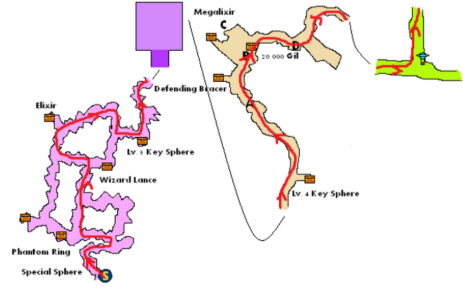
\includegraphics{graphics/sinpath}
	\item Before Seymour Omnis, \formation{\tidus}{\auron}{\yuna}
	\item Go up the steps, \sd
\end{enumerate}
\vfill
\begin{battle}[80000]{Seymour Omnis}
	\begin{itemize}
		\yunaf Defend
		\tidusf Armor Break
		\item \textit{If Armor Break Hit:}
		      \begin{itemize}
			      \auronf Defend
			      \summon{\bahamut}
			      \bahamutf Attack
		      \end{itemize}
		\item \textit{If Armor Break Missed:}
		      \begin{itemize}
			      \switch{\auron}{\rikku}
			      \rikkuf \od\ Mix Spherimorph Throwable + HiPot/MegaPot/XPot/Mega Phoenix
			      \yunaf Cure Mortiphasm
			      \tidusf Armor Break
			      \summon{\bahamut}
			      \bahamutf Attack
		      \end{itemize}
	\end{itemize}
\end{battle}
\begin{enumerate}[resume]
	\item \sd, walk north.
	\item \formation{\tidus}{\kimahri}{\auron}
	\item Make sure that \rikku's \od\ is charged. Can skip if using Skill Sphere for Armor Break.
	\item Turn left onto the bridge, go onto the next screen. \save\ if needed.
	\item Complete the minigame, picking up the eggs and avoiding the crystals.
\end{enumerate}
\vfill
\ 
\end{multicols}
\begin{spheregrid}
	\begin{multicols}{2}
		\begin{itemize}
			\item \textit{If you got 2 or 4 \textbf{Return Spheres}:}
			      \begin{itemize}
				      \yunaf Attribute Sphere \rikku's +3 Agi (hold L)
				      \item Return Sphere ($\downarrow \downarrow \leftarrow \leftarrow$) or Friend Sphere ($\downarrow \leftarrow$) there
				      \item Go down, picking up Agi+4, Spare Change, Agi+4
			      \end{itemize}
			      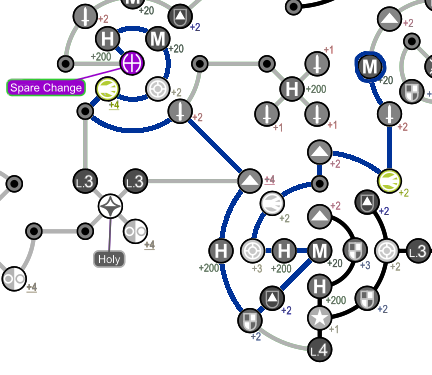
\includegraphics[width=.8\columnwidth]{graphics/4_Return_final_grid}
			\item \textit{If you got 0 \textbf{Return Spheres}:}
			      \begin{itemize}
				      \item Spare Change
				      \item Move $\swarrow$
				      \item Agi+4
				      \item Attribute Sphere Agi+3 at the start of \rikku\'s grid
				      \item Move to Mug $\searrow\rightarrow x7$
				      \item Agi+4
				      \item Move $\downarrow$
				      \item Agi+4
			      \end{itemize}
			      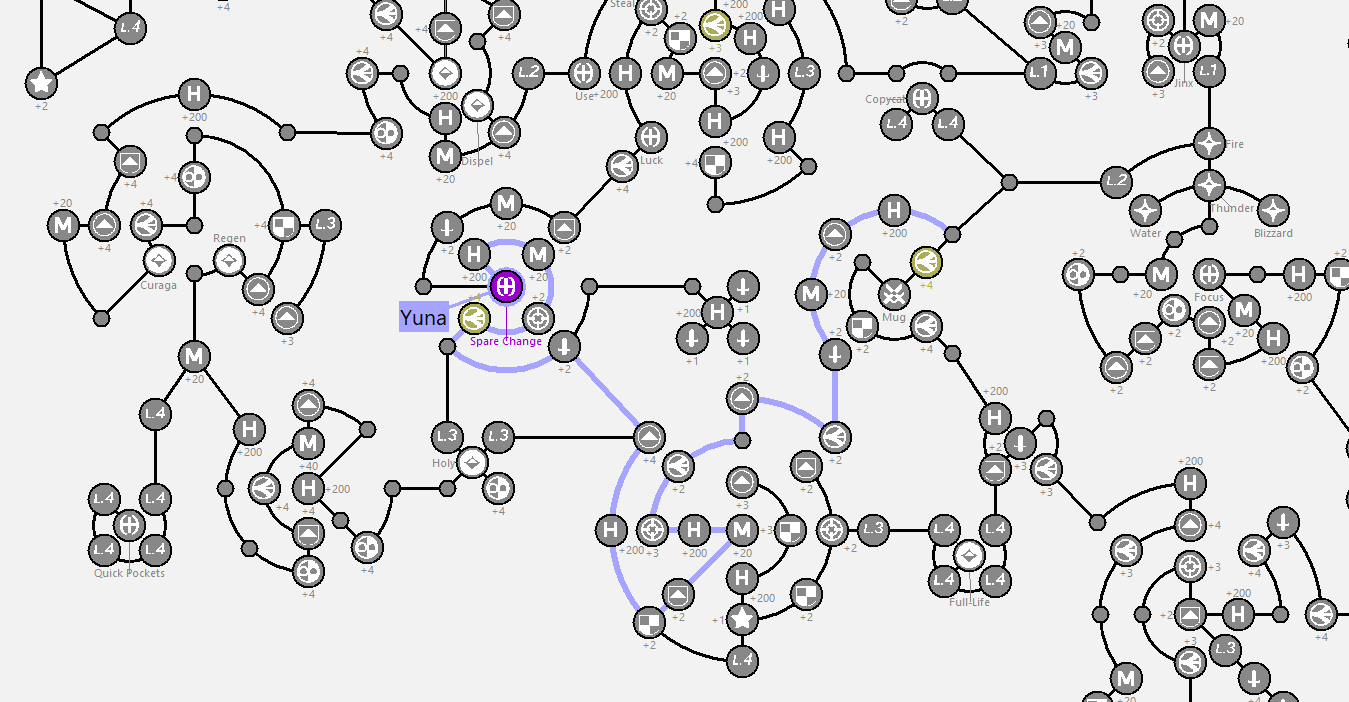
\includegraphics[width=.8\columnwidth]{graphics/0_return_before_BFA}
			      \columnbreak
			      \tidusf \textit{If you didn't get a \textbf{Zombie Strike} weapon}:
			      \begin{itemize}
				      \item \textit{If you got 2 or 4 \textbf{Return Spheres}:}
				            \begin{itemize}
					            \item Return $\uparrow\leftarrow$
					            \item Move $\uparrow$
					            \item Level 4 Keysphere
					            \item Move $\uparrow$
					            \item Zombie Attack
				            \end{itemize}
				      \item \textit{If you got 0 \textbf{Return Spheres}:}
				            \begin{itemize}
					            \item Move $\uparrow x5$
					            \item Level 4 Keysphere
					            \item Move $\uparrow$
					            \item Zombie Attack
				            \end{itemize}
						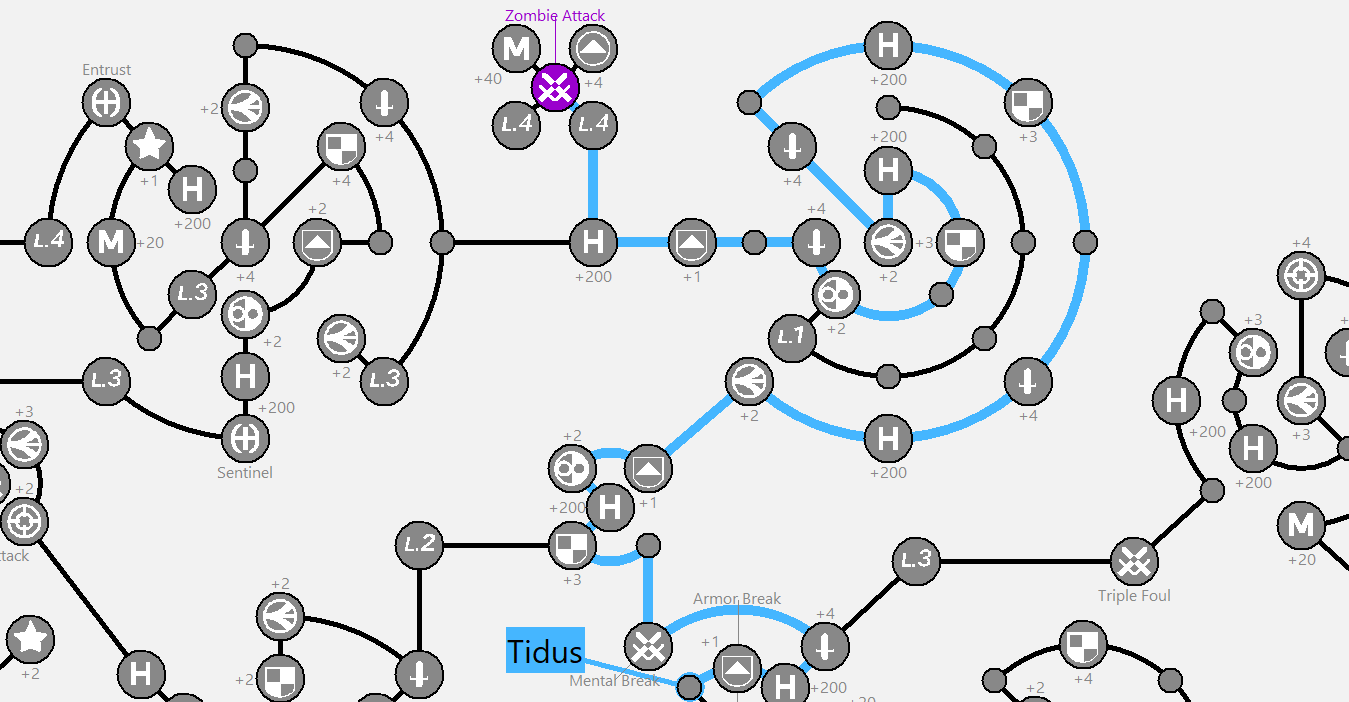
\includegraphics[width=.8\columnwidth]{graphics/Tidus_BFA}
			      \end{itemize}
				            \rikkuf If no \od, use Skill Sphere to learn Armor Break
		\end{itemize}
	\end{multicols}
\end{spheregrid}
\begin{multicols}{2}
	\begin{equip}
		\begin{itemize}
			\item Anyone that isn't \tidus, \yuna, \auron:
			      \begin{itemize}
				      \item Equip Zombie Strike Weapon
			      \end{itemize}
		\end{itemize}
	\end{equip}
	\begin{enumerate}[resume]
		\item Walk up to Jecht, \cs[4:30]
	\end{enumerate}
	\vfill
	\begin{battle}[180000]{Braska's Final Aeon}
		\begin{itemize}
			\switch{\yuna}{\rikku}
			\rikkuf \od\ Mix Grenade + HP Sphere or Armor Break
			\tidusf Talk
			\switch{\auron}{\yuna}
			\summon{\bahamut}
			\bahamutf Attack
		\end{itemize}
	\end{battle}
\end{multicols}
\begin{enumerate}[resume]
	\item \cs+\skippablefmv[4:00]
\end{enumerate}
\begin{battle}{Possessed  Aeons}
	\begin{itemize}
		\item Spare Change as follows:
		      \begin{itemize}
			      \valeforf \num{20000} Gil
			      \ifritf \num{30000} Gil
			      \ixilonf \num{30000} Gil
			      \bahamutf \num{40000} Gil
			      \shivaf All Remaining Gil
		      \end{itemize}
	\end{itemize}
\end{battle}
\begin{enumerate}[resume]
	\item \cs[1:40]
\end{enumerate}
\begin{battle}[99999]{Yu Yevon}
	\begin{itemize}
		\item Zombie Attack:
		      \begin{itemize}
			      \yunaf Defend
			      \tidusf Zombie Attack
		      \end{itemize}
		\item \yuna\ Zombie Strike Weapon:
			\begin{itemize}
				\yunaf Switch Weapon
				\tidusf Switch Weapon
				\yunaf Attack
				\tidusf Phoenix Down Yu Yevon
			\end{itemize}
		\item \tidus\ Zombie Strike Weapon:
		      \begin{itemize}
			      \yunaf Defend
			      \tidusf Change Weapon
			      \tidusf Attack
		      \end{itemize}
		\item \rikku\ Zombie Strike Weapon:
		      \begin{itemize}
			      \yunaf Defend
			      \tidusf Haste \rikku
			      \yunaf Change Weapon
			      \rikkuf Attack
		      \end{itemize}
		\item \auron\ Zombie Strike Weapon:
			\begin{itemize}
				\switch{\yuna}{\auron}
				\auronf Change Weapon
				\tidusf Defend
				\auronf Attack
			\end{itemize}
		\item Anyone Else Zombie Strike Weapon:
		      \begin{itemize}
			      \switch{\yuna}{character with Zombie Strike Weapon}
			      \item That Character: Attack
			            \tidusf Phoenix Down Yu Yevon
		      \end{itemize}

		      \item Anyone: Phoenix Down Yu Yevon
	\end{itemize}
\end{battle}
\bothvfill
\begin{multicols}{2}
\colend

\end{document}